\documentclass[12pt,a4paper]{report}

% ============================ ENCODAGE / LANGUE / POLICE ===================
\usepackage{iftex}
\ifPDFTeX
  \usepackage[utf8]{inputenc}
  \usepackage[T1]{fontenc}
\else                                   % XeLaTeX / LuaLaTeX : police système
  \usepackage{fontspec}
  \setmainfont{Times New Roman}
\fi
\usepackage[french]{babel}

% ============================ MISE EN PAGE ================================
\usepackage[a4paper,margin=2.5cm,headheight=14pt]{geometry}
\usepackage{graphicx}
\graphicspath{{figures/}}
\usepackage{xcolor}
\usepackage{tikz}
\usetikzlibrary{arrows.meta, positioning, shapes.geometric, calc, fit, backgrounds}
\usepackage{booktabs}
\usepackage{array}
\usepackage{longtable}
\usepackage{multirow}
\usepackage{enumitem}
\usepackage{amsmath, amssymb}
\usepackage{caption}
\usepackage{subcaption}
\usepackage{fancyhdr}
\usepackage{listings}
\usepackage{titlesec}
\usepackage[hidelinks]{hyperref}

% ============================ COULEURS (app PrognoSense) ==================
\definecolor{psbleu}{RGB}{0,140,170}
\definecolor{psbleud}{RGB}{0,90,115}
\definecolor{psvert}{RGB}{0,150,100}
\definecolor{psambre}{RGB}{210,150,30}
\definecolor{psgris}{RGB}{70,80,90}
\definecolor{psrouge}{RGB}{200,60,60}
\definecolor{pscode}{RGB}{245,247,249}

\hypersetup{
  colorlinks=true, linkcolor=psbleud, citecolor=psvert,
  urlcolor=psbleu, linktoc=all,
}

% ============================ EN-TÊTES ===================================
\pagestyle{fancy}
\fancyhf{}
\setlength{\headheight}{14pt}
\lhead{\small\color{psgris}\textsc{PrognoSense}}
\rhead{\small\color{psgris}\leftmark}
\cfoot{\thepage}
\renewcommand{\headrulewidth}{0.4pt}
\renewcommand{\chaptermark}[1]{\markboth{\thechapter.\ #1}{}}

% ============================ TITRES =====================================
\titleformat{\chapter}[display]
  {\normalfont\huge\bfseries\color{psbleu}}
  {\filright\Large\color{psgris}\chaptername\ \thechapter}{0.6em}{\Huge}
\titlespacing*{\chapter}{0pt}{10pt}{24pt}
\titleformat{\section}{\Large\bfseries\color{psbleud}}{\thesection}{0.6em}{}
\titleformat{\subsection}{\large\bfseries\color{psgris}}{\thesubsection}{0.6em}{}

% ============================ CODE =======================================
\definecolor{kw}{RGB}{0,90,140}
\definecolor{cmt}{RGB}{110,120,130}
\definecolor{str}{RGB}{0,130,90}
\lstdefinestyle{ps}{
  basicstyle=\ttfamily\footnotesize,
  keywordstyle=\color{kw}\bfseries,
  commentstyle=\color{cmt}\itshape,
  stringstyle=\color{str},
  breaklines=true, frame=single, rulecolor=\color{psgris!35},
  backgroundcolor=\color{pscode}, columns=fullflexible,
  keepspaces=true, showstringspaces=false, captionpos=b,
  numbers=left, numberstyle=\tiny\color{psgris}, numbersep=7pt,
}
\lstset{style=ps}
\renewcommand{\lstlistingname}{Extrait de code}

\captionsetup{font=small, labelfont={bf,color=psbleud}}

\begin{document}

% ===================================================================
% PAGE DE GARDE
% ===================================================================
\begin{titlepage}
\centering
\thispagestyle{empty}
\vspace*{0.5cm}


\includegraphics[width=0.9\textwidth,height=4cm]{logo_ensam.jpg}\\[0.5cm]

{\color{psgris!40}\rule{0.9\textwidth}{0.4pt}}\\[0.4cm]

{\large\bfseries École Nationale Supérieure d'Arts et Métiers --- Meknès}\\[0.4cm]
{\small\itshape Université Moulay Ismaïl}\\[0.32cm]
{\normalsize Filière : Intelligence Artificielle et Technologies des données -- Systèmes Industriels}

\vfill

\begin{tikzpicture}
  \draw[psbleu, line width=2pt] (0,0) rectangle (15,0.09);
\end{tikzpicture}\\[0.8cm]

{\small\itshape Rapport de Projet --- Maintenance Industrielle et Prédictive}\\[0.7cm]

\begin{tikzpicture}
  \node[rectangle, rounded corners=10pt, fill=psbleu!12, draw=psbleu, line width=1.6pt,
        minimum width=14cm, minimum height=4.1cm, text centered] {
    \begin{minipage}{13cm}\centering
      {\fontsize{42}{46}\selectfont\bfseries\color{psbleu} PrognoSense}\\[0.5cm]
      {\Large\color{psgris} Plateforme Intelligente de Maintenance Prédictive\\[0.15cm]
      basée sur l'Analyse Vibratoire et l'Intelligence Artificielle}
    \end{minipage}
  };
\end{tikzpicture}\\[1.2cm]

\begin{tikzpicture}
  \draw[psambre, line width=1.6pt] (0,0) rectangle (15,0.07);
\end{tikzpicture}

\vfill

\noindent
\begin{minipage}[t]{0.48\textwidth}
  \raggedright
  {\large\bfseries Réalisé par :}\\[0.45cm]
  {\Large Souleymane DIALLO}
\end{minipage}%
\hfill
\begin{minipage}[t]{0.48\textwidth}
  \raggedleft
  {\large\bfseries Encadré par :}\\[0.45cm]
  {\Large Pr. Zaki SMAIL}
\end{minipage}

\vspace{0.9cm}
\begin{tikzpicture}
  \draw[psgris!50, line width=0.5pt] (0,0) -- (15,0);
\end{tikzpicture}\\[0.25cm]
{\small Année universitaire 2025--2026}
\end{titlepage}

% ===================================================================
% RÉSUMÉ / ABSTRACT
% ===================================================================
\pagenumbering{roman}
\chapter*{Résumé}
\addcontentsline{toc}{chapter}{Résumé}
\markboth{Résumé}{}

La maintenance représente aujourd'hui un poste de coût majeur de l'industrie, et les
arrêts non planifiés en constituent la part la plus pénalisante. Ce projet présente
\textbf{PrognoSense}, une plateforme logicielle complète de \textbf{maintenance prédictive
industrielle} qui transforme l'analyse des signaux vibratoires en décisions de maintenance
anticipées et chiffrées.

La plateforme met en œuvre l'intégralité de la chaîne de surveillance conditionnelle :
acquisition de signaux (rééchantillonnage à 12{,}8\,kHz, fenêtrage glissant), extraction
d'indicateurs temporels et fréquentiels (RMS, kurtosis, facteur de crête, énergies par
bande, entropie spectrale), diagnostic spectral des défauts (fréquences caractéristiques
de roulements BPFO/BPFI/BSF/FTF, analyse d'enveloppe par transformée de Hilbert),
évaluation de la sévérité selon la norme \textbf{ISO~10816/20816} (vitesse vibratoire en
mm/s, zones A/B/C/D), détection d'anomalies non supervisée par auto-encodeur, classification
des défauts et pronostic de durée de vie restante (RUL).

Cinq modèles d'apprentissage automatique (Decision Tree, Random Forest, XGBoost, MLP,
Huber) ont été entraînés et comparés sur \textbf{quatre jeux de données de référence}
totalisant plus de \textbf{66~000 fenêtres} : VBL-VA001 (100\,\% d'exactitude), CWRU
(97{,}6\,\% avec XGBoost sur 10 classes), Mechanical Faults (89{,}6\,\% avec le MLP) et
CMAPSS pour la régression RUL (MAE de \textbf{9{,}61 cycles}, $R^2=0{,}90$ avec XGBoost).
La méthodologie d'évaluation repose sur un découpage \emph{par fichier source} interdisant
toute fuite de données.

Au-delà du diagnostic, PrognoSense intègre une couche d'\textbf{industrialisation et de
confiance} : connecteurs terrain (OPC-UA, MQTT) alimentant une couche d'ingestion
universelle, apprentissage du comportement sain \emph{propre à chaque machine}, indicateurs
de fiabilité \emph{mesurés} (MTBF, MTTR, disponibilité, ROI), création automatique d'ordres
de travail transmis à la GMAO, journal d'audit horodaté, versioning des modèles avec retour
arrière, mesure du taux réel de fausses alarmes, et un \textbf{copilot} à base de modèle de
langage ancré sur une base de connaissances normative (RAG). L'architecture est conçue pour
passer à l'échelle (base time-series TimescaleDB).

\vspace{0.4cm}
\noindent\textbf{Mots-clés :} maintenance prédictive, analyse vibratoire, ISO~10816,
détection d'anomalies, auto-encodeur, RUL, CMAPSS, CWRU, XGBoost, OPC-UA, GMAO,
explicabilité, MLOps, FastAPI, React.

\vspace{0.8cm}
\begin{center}{\color{psbleu}\rule{0.5\textwidth}{0.6pt}}\end{center}
\vspace{0.4cm}

\begin{center}\textbf{\large Abstract}\end{center}

Maintenance is a major cost center in industry, and unplanned downtime is its most
penalizing component. This project introduces \textbf{PrognoSense}, a comprehensive
software platform for \textbf{industrial predictive maintenance} that turns vibration
signal analysis into anticipated, quantified maintenance decisions.

The platform implements the full condition-based maintenance pipeline: signal acquisition
(resampling to 12.8\,kHz, sliding windows), extraction of time- and frequency-domain
indicators (RMS, kurtosis, crest factor, band energies, spectral entropy), spectral fault
diagnosis (bearing characteristic frequencies BPFO/BPFI/BSF/FTF, Hilbert envelope
analysis), severity assessment per the \textbf{ISO~10816/20816} standard (vibration
velocity in mm/s, zones A/B/C/D), unsupervised anomaly detection via an autoencoder, fault
classification and Remaining Useful Life (RUL) prognosis.

Five machine-learning models were trained and benchmarked on \textbf{four reference
datasets} totalling more than \textbf{66{,}000 windows}: VBL-VA001 (100\,\% accuracy),
CWRU (97.6\,\% with XGBoost over 10 classes), Mechanical Faults (89.6\,\% with the MLP) and
CMAPSS for RUL regression (MAE of \textbf{9.61 cycles}, $R^2=0.90$ with XGBoost), using a
leakage-free split by source file.

Beyond diagnosis, PrognoSense adds an \textbf{industrialization and trust} layer: field
connectors (OPC-UA, MQTT) feeding a universal ingestion endpoint, per-machine healthy
baseline learning, \emph{measured} reliability indicators (MTBF, MTTR, availability, ROI),
automatic work-order generation pushed to the CMMS, a timestamped audit trail, model
versioning with rollback, real false-alarm-rate measurement, and an LLM-based
\textbf{copilot} grounded on a normative knowledge base (RAG). The architecture is designed
to scale on a TimescaleDB time-series backend.

\vspace{0.3cm}
\noindent\textbf{Keywords:} predictive maintenance, vibration analysis, ISO~10816, anomaly
detection, autoencoder, RUL, CMAPSS, CWRU, XGBoost, OPC-UA, CMMS, explainability, MLOps.


\cleardoublepage
\tableofcontents
\listoffigures
\listoftables

\cleardoublepage
\pagenumbering{arabic}

% ===================================================================
% CHAPITRES
% ===================================================================
\chapter{Introduction}

\section{Contexte industriel}
La disponibilité des équipements est un facteur déterminant de la compétitivité
industrielle. Dans une usine, une heure d'arrêt d'une ligne de production peut coûter
plusieurs milliers d'euros, et les défaillances de machines tournantes (pompes,
ventilateurs, compresseurs, réducteurs, turbines) figurent parmi les causes les plus
fréquentes d'indisponibilité. Or, plus de la moitié de ces défaillances sont d'origine
mécanique et se manifestent, des semaines voire des mois à l'avance, par une évolution
caractéristique du comportement vibratoire de la machine.

On distingue traditionnellement trois stratégies de maintenance :
\begin{itemize}[leftmargin=1.5em]
  \item la \textbf{maintenance corrective}, qui intervient après la panne. Simple à
        organiser, elle est la plus coûteuse : arrêt subi, dégâts collatéraux, perte de
        production, risque sécurité.
  \item la \textbf{maintenance préventive systématique}, qui intervient à intervalles
        fixes (calendaires ou à compteur). Elle réduit les pannes mais engendre un
        gaspillage : on remplace des composants encore sains, et l'on n'élimine pas les
        défaillances précoces survenant entre deux interventions.
  \item la \textbf{maintenance prédictive} (ou conditionnelle, \emph{Condition-Based
        Maintenance}, CBM), qui intervient \emph{au bon moment}, en fonction de l'état
        réel de la machine mesuré en continu. C'est la stratégie la plus efficiente, mais
        aussi la plus exigeante techniquement.
\end{itemize}

La maintenance prédictive repose sur un principe simple : une machine qui se dégrade
\og parle \fg{} à travers ses signaux physiques (vibration, température, courant,
acoustique). L'enjeu est de \emph{savoir l'écouter} : capter ces signaux, en extraire des
indicateurs pertinents, reconnaître les signatures de défaut, et estimer le temps restant
avant la défaillance.

\section{Problématique}
La mise en œuvre d'une solution de maintenance prédictive crédible se heurte à plusieurs
difficultés concrètes :
\begin{enumerate}[leftmargin=1.6em]
  \item \textbf{Détecter tôt} une dégradation, alors que ses premières manifestations sont
        noyées dans le bruit et masquées par les conditions d'exploitation variables.
  \item \textbf{Diagnostiquer précisément} le type de défaut (balourd, désalignement,
        défaut de roulement, jeu mécanique, défaut d'engrenage) pour orienter
        l'intervention.
  \item \textbf{Quantifier} l'état de santé et la durée de vie restante de façon
        exploitable pour la planification.
  \item \textbf{Maîtriser le taux de fausses alarmes} : un système qui alerte à tort
        perd la confiance des équipes et finit désactivé.
  \item \textbf{Rendre la solution actionnable et traçable} : transformer une alerte en
        intervention planifiée, et pouvoir justifier chaque décision a posteriori.
\end{enumerate}

À ces difficultés techniques s'ajoute une contrainte de \emph{crédibilité industrielle} :
les indicateurs et diagnostics produits doivent parler le langage normalisé des ingénieurs
de fiabilité (zones de sévérité ISO, MTBF, MTTR, disponibilité) plutôt que des métriques
propriétaires non vérifiables.

\section{Objectifs du projet}
L'objectif est de concevoir et de réaliser une plateforme logicielle complète, nommée
\textbf{PrognoSense}, qui couvre l'ensemble de la chaîne de maintenance prédictive :
\begin{itemize}[leftmargin=1.5em]
  \item acquérir et traiter des signaux vibratoires issus de plusieurs natures de machines ;
  \item extraire des indicateurs physiquement interprétables et diagnostiquer les défauts ;
  \item entraîner, comparer et sélectionner des modèles d'apprentissage automatique de
        classification de défauts et de pronostic de durée de vie ;
  \item détecter des anomalies inconnues par apprentissage non supervisé ;
  \item évaluer la sévérité selon la norme ISO~10816/20816 ;
  \item synthétiser un \emph{indice de santé} et suivre la flotte en temps réel ;
  \item transformer les alertes en ordres de travail transmissibles à une GMAO ;
  \item mesurer la fiabilité réelle (MTBF, MTTR, disponibilité, ROI, fausses alarmes) ;
  \item garantir la confiance : explicabilité, calibration, audit, versioning des modèles ;
  \item exposer le tout via une interface web ergonomique et un copilot conversationnel.
\end{itemize}

\section{Démarche et organisation du rapport}
La démarche a suivi une progression incrémentale : maîtrise du pipeline de traitement du
signal et des données, entraînement et benchmark des modèles, construction de la plateforme
applicative (backend/frontend), puis industrialisation (normes, connectivité, boucle
fermée, confiance).

Le rapport est organisé comme suit. Le chapitre~\ref{chap:etatart} présente l'état de l'art
de la maintenance prédictive et le positionnement vis-à-vis des solutions du marché. Le
chapitre~\ref{chap:datasets} analyse les jeux de données utilisés. Le
chapitre~\ref{chap:archi} décrit l'architecture générale. Le chapitre~\ref{chap:pipeline}
détaille le pipeline de traitement du signal et l'extraction des indicateurs. Le
chapitre~\ref{chap:bench} présente le benchmark des cinq modèles. Le
chapitre~\ref{chap:anomalie} traite la détection d'anomalies. Les
chapitres~\ref{chap:backend} et~\ref{chap:frontend} décrivent respectivement le backend et
le frontend. Le chapitre~\ref{chap:indus} couvre l'industrialisation (ISO, connectivité,
GMAO, KPIs réels, copilot, confiance). Le chapitre~\ref{chap:defis} relate les défis
techniques rencontrés. Le chapitre~\ref{chap:resultats} synthétise et interprète les
résultats. Le chapitre~\ref{chap:limites} discute les limites et perspectives, et le
chapitre~\ref{chap:conclusion} conclut.

\chapter{État de l'art et positionnement}
\label{chap:etatart}

\section{La maintenance conditionnelle et l'architecture OSA-CBM}
La maintenance conditionnelle s'appuie sur une chaîne de traitement standardisée par la
norme \textbf{ISO~13374}, connue sous le nom d'architecture \textbf{OSA-CBM} (\emph{Open
System Architecture for Condition-Based Maintenance}). Cette architecture décompose le
processus en couches fonctionnelles successives :
\begin{enumerate}[leftmargin=1.6em]
  \item \textbf{Data Acquisition} (DA) : acquisition des signaux bruts.
  \item \textbf{Data Manipulation} (DM) : traitement du signal, extraction d'indicateurs.
  \item \textbf{State Detection} (SD) : comparaison à des seuils, détection d'anomalies.
  \item \textbf{Health Assessment} (HA) : évaluation de l'état de santé global.
  \item \textbf{Prognostics} (PA) : pronostic, estimation de la durée de vie restante.
  \item \textbf{Advisory Generation} (AG) : génération de recommandations et d'actions.
\end{enumerate}
PrognoSense reprend fidèlement cette décomposition : l'ingestion (DA), l'extraction
d'indicateurs (DM), la détection d'anomalies et le seuillage (SD), l'indice de santé (HA),
le pronostic RUL (PA) et la génération d'ordres de travail (AG).

\section{Techniques d'analyse vibratoire}
L'analyse vibratoire est l'outil de diagnostic privilégié des machines tournantes car
chaque mode de défaillance produit une \emph{signature} reconnaissable :
\begin{itemize}[leftmargin=1.5em]
  \item \textbf{Analyse temporelle} : des descripteurs statistiques (RMS, kurtosis, facteur
        de crête) caractérisent l'énergie et le caractère impulsif du signal. Le kurtosis
        et le facteur de crête sont particulièrement sensibles aux chocs répétés des défauts
        de roulement naissants.
  \item \textbf{Analyse fréquentielle} : la transformée de Fourier (FFT) révèle les
        composantes spectrales. Le balourd se manifeste à la fréquence de rotation
        ($1\times$), le désalignement à $2\times$, le jeu mécanique par une multiplicité
        d'harmoniques.
  \item \textbf{Fréquences caractéristiques de roulement} : BPFO (bague externe), BPFI
        (bague interne), BSF (billes), FTF (cage), calculées à partir de la géométrie du
        roulement et de la vitesse de rotation.
  \item \textbf{Analyse d'enveloppe} : la démodulation par transformée de Hilbert d'une
        bande de résonance haute fréquence fait ressortir les défauts de roulement masqués
        dans le spectre brut.
\end{itemize}

\section{Apprentissage automatique pour le diagnostic et le pronostic}
Au-delà du diagnostic expert manuel, l'apprentissage automatique permet d'automatiser la
reconnaissance des défauts (classification supervisée) et l'estimation de la durée de vie
restante (régression). Les approches non supervisées (auto-encodeurs, méthodes de détection
d'anomalies) complètent ce dispositif en repérant les comportements \emph{inconnus}, non
présents dans les données d'entraînement --- un atout décisif, puisqu'une partie importante
des défaillances industrielles relèvent de modes rares ou imprévus.

\section{Normes applicables}
Le domaine est fortement encadré par des normes que PrognoSense intègre explicitement :
\begin{itemize}[leftmargin=1.5em]
  \item \textbf{ISO~10816 / 20816} : évaluation de la sévérité vibratoire par la vitesse
        efficace (mm/s) et classement en zones A/B/C/D selon la classe de machine.
  \item \textbf{ISO~13374} : architecture de traitement OSA-CBM (ci-dessus).
  \item \textbf{ISO~13373} : surveillance et diagnostic vibratoire.
  \item \textbf{ISO~13381} : pronostic.
  \item \textbf{ISO~18436} : qualification des analystes vibratoires (catégories I à IV).
\end{itemize}

\section{Solutions du marché et positionnement de PrognoSense}
Le marché de la maintenance prédictive est occupé par des acteurs établis : SKF
(Enlight, @ptitude), Emerson (AMS, Plantweb), GE Bently Nevada (System~1), Brüel \& Kjær,
ainsi que des acteurs plus récents centrés sur l'IA et les capteurs sans fil (Augury,
AspenTech~Mtell, Siemens~Senseye, Schaeffler~OPTIME). Ces solutions sont puissantes mais
présentent des limites récurrentes : matériel propriétaire, coût de licence élevé,
fermeture (peu d'interopérabilité), et fréquemment un caractère de \og boîte noire \fg{}
peu explicable.

PrognoSense ne vise pas à rivaliser en largeur fonctionnelle avec ces suites, mais à
occuper un positionnement différenciant, articulé autour de cinq axes :
\begin{enumerate}[leftmargin=1.6em]
  \item \textbf{Ouverture} : connectable à n'importe quel capteur via les protocoles
        standards (OPC-UA, MQTT), sans verrouillage propriétaire.
  \item \textbf{Diagnostic normalisé} : sévérité exprimée en zones ISO~10816, défendable
        par un ingénieur de fiabilité.
  \item \textbf{Explicabilité et confiance} : importance des indicateurs, calibration,
        journal d'audit, taux de fausses alarmes mesuré.
  \item \textbf{Copilot ancré} : assistant en langage naturel dont les réponses citent
        les sources normatives (RAG).
  \item \textbf{Boucle fermée} : de l'alerte à l'ordre de travail transmis à la GMAO.
\end{enumerate}
Ce positionnement guide l'ensemble des choix de conception détaillés dans les chapitres
suivants.

\chapter{Analyse des jeux de données}
\label{chap:datasets}

Le choix des données conditionne la pertinence d'une solution de maintenance prédictive.
Plutôt que de se limiter à un seul cas, le projet s'appuie sur \textbf{cinq jeux de données
de référence}, couvrant des natures de machines, des modalités d'acquisition et des tâches
différentes. Cette diversité valide le caractère \emph{générique} du pipeline.

\section{Vue comparative}
Le tableau~\ref{tab:datasets} synthétise les caractéristiques techniques réelles des
datasets après traitement (dimensions effectives mesurées sur les tenseurs produits).

\begin{table}[h]
\centering
\small
\caption{Caractéristiques des jeux de données utilisés (valeurs réelles après pipeline).}
\label{tab:datasets}
\begin{tabular}{>{\bfseries}l c c c c c}
\toprule
Dataset & Tâche & Fréq. éch. & Canaux & Fenêtres & Features \\
\midrule
VBL-VA001         & Classif. (4 cl.)  & 20\,kHz   & 3 (x,y,z) & 400    & 45  \\
CWRU              & Classif. (10 cl.) & 12\,kHz   & 1 (DE)    & 12\,627 & 15  \\
Mechanical Faults & Classif. (4 cl.)  & 25\,kHz   & 4         & 36\,000 & 132 \\
CMAPSS FD001      & Régression (RUL)  & cycles    & 21 capt.  & 17\,731 & 126 \\
MCC5-THU          & Classif. (8 cl.)  & 12{,}8\,kHz & 3 (x,y,z) & ---    & ---  \\
\bottomrule
\end{tabular}
\end{table}

\section{VBL-VA001 --- bancs d'essai vibratoires}
Ce jeu de données fournit des signaux tri-axiaux (x, y, z) échantillonnés à 20\,kHz sur un
banc d'essai, répartis en \textbf{quatre classes parfaitement équilibrées} (100 fenêtres
chacune) : \texttt{normal}, \texttt{bearing} (roulement), \texttt{misalignment}
(désalignement) et \texttt{unbalance} (balourd). Après extraction, chaque fenêtre est
décrite par \textbf{45 features} (15 par canal). Sa petite taille (400 fenêtres) et la
séparabilité nette de ses classes en font un cas \emph{facile}, idéal pour valider le
pipeline de bout en bout.

\section{CWRU --- défauts de roulement (Case Western Reserve University)}
Référence académique mondiale du diagnostic de roulement, CWRU fournit des signaux
d'accélération (canal \texttt{DE\_time}, côté entraînement) échantillonnés à 12\,kHz. Le
projet en retient une taxonomie fine à \textbf{10 classes} croisant la \emph{localisation}
du défaut (bague interne, bague externe, bille) et sa \emph{sévérité} (faible, moyen,
grave), plus l'état sain :
\begin{center}\small\ttfamily
sain, roulement\_interne\_\{faible,moyen,grave\}, roulement\_externe\_\{faible,moyen,grave\},
roulement\_bille\_\{faible,moyen,grave\}
\end{center}
Le dataset traité compte \textbf{12\,627 fenêtres} et \textbf{15 features} (un seul canal).
La classe \texttt{sain} domine (3\,531 fenêtres) tandis que les neuf classes de défaut
comptent environ 1\,010 fenêtres chacune. Cette granularité (localisation + sévérité)
rend la tâche réaliste et exigeante.

\section{Mechanical Faults --- machine tournante multi-capteurs}
Ce jeu de données provient d'un banc de machine tournante instrumenté de \textbf{4
accéléromètres} (vertical et horizontal, côté poulie et côté disque), échantillonnés à
25\,kHz. Quatre classes équilibrées de \textbf{9\,000 fenêtres} chacune (36\,000 au total)
sont considérées : \texttt{sain}, \texttt{desalignement}, \texttt{desequilibre} et
\texttt{jeu\_mecanique}. La richesse multi-capteurs et la finesse spectrale conduisent à un
vecteur de \textbf{132 features} (33 par canal, dont des descripteurs harmoniques et
d'enveloppe spécialisés). C'est le dataset le plus volumineux et le plus difficile pour la
classification (cf. chapitre~\ref{chap:bench}).

\section{CMAPSS FD001 --- pronostic de durée de vie (NASA)}
CMAPSS (\emph{Commercial Modular Aero-Propulsion System Simulation}) est la référence du
\textbf{pronostic de RUL}. Le sous-ensemble FD001 simule la dégradation de \textbf{100
moteurs} jusqu'à la panne, chacun suivi par \textbf{21 capteurs} au fil des cycles de
fonctionnement. Le projet en dérive \textbf{17\,731 fenêtres} décrites par \textbf{126
features} (statistiques sur fenêtres de cycles des 21 capteurs). La cible principale est la
RUL (durée de vie restante, plafonnée à 125 cycles, moyenne $\approx 80{,}6$). Des labels de
dégradation (\texttt{sain}, \texttt{degradation\_precoce}, \texttt{degradation\_avancee},
\texttt{critique}) sont également dérivés pour la détection d'anomalies. À noter : les
données brutes comportaient 119\,362 valeurs manquantes (capteurs constants), traitées par
remplacement à zéro lors du benchmark.

\section{MCC5-THU --- défauts d'engrenage}
Ce jeu de données de réducteur (gearbox), échantillonné à 12{,}8\,kHz sur 3 axes, comporte
\textbf{huit classes} de défauts d'engrenage : sain, \texttt{pitting} (piqûres),
\texttt{usure}, \texttt{dent\_cassee}, \texttt{fissure}, \texttt{dent\_manquante} et deux
défauts \emph{mixtes} (rupture de dent combinée à un défaut de roulement interne/externe).
Il est traité par un \textbf{réseau de neurones convolutif 1D} (CNN) opérant directement sur
le signal, sans extraction manuelle de features (cf. chapitre~\ref{chap:bench}).

\section{Pipeline d'unification}
La diversité des formats (CSV, MAT, TXT, multi-canaux, fréquences hétérogènes) est absorbée
par un \textbf{adaptateur unifié} (\texttt{DatasetAdapter}) qui produit une structure
commune \texttt{UnifiedSignal}. Les opérations clés sont : le \textbf{rééchantillonnage} à
une fréquence cible de 12\,800\,Hz (\texttt{resample\_poly}), la \textbf{normalisation}
Z-score par canal, et le \textbf{fenêtrage glissant} (fenêtres de 1\,024 points, recouvrement
de 50\,\%). Un mécanisme de cache (clé MD5 sur chemin + configuration) évite de recalculer
les features. Cette abstraction est ce qui permet au même pipeline de traiter indifféremment
un roulement CWRU et un turbomoteur CMAPSS.

\section{Couverture des modes de défaillance : un spectre complet}
\label{sec:couverture}
Le véritable apport du choix des données réside dans leur \textbf{complémentarité}. Là où
la plupart des travaux académiques se concentrent sur un \emph{unique} dataset et une
\emph{unique} tâche (typiquement la classification CWRU), PrognoSense couvre l'ensemble du
spectre des défaillances des machines tournantes industrielles. Le
tableau~\ref{tab:fautes} recense les \textbf{modes de défaillance réellement intégrés} et
diagnosticables par la plateforme.

\begin{table}[h]
\centering\small
\caption{Catalogue des modes de défaillance couverts par PrognoSense.}
\label{tab:fautes}
\begin{tabular}{>{\bfseries}p{3.4cm} p{6.4cm} p{3.6cm}}
\toprule
Famille de défaut & Modes couverts & Source / signature \\
\midrule
Balourd (déséquilibre) & déséquilibre rotor & VBL, MF --- pic $1\times$ \\
Désalignement & parallèle / angulaire & VBL, MF --- pics $2\times$, $3\times$ \\
Jeu mécanique & desserrage, jeu de palier & MF --- harmoniques multiples \\
Roulement --- bague externe & faible / moyen / grave & CWRU --- BPFO + enveloppe \\
Roulement --- bague interne & faible / moyen / grave & CWRU --- BPFI + bandes latérales \\
Roulement --- bille & faible / moyen / grave & CWRU --- BSF + FTF \\
Engrenage --- piqûres & \texttt{pitting} & MCC5 --- GMF + sidebands \\
Engrenage --- usure & usure de denture & MCC5 \\
Engrenage --- dent & dent cassée, fissurée, manquante & MCC5 \\
Défauts mixtes & rupture de dent + roulement int./ext. & MCC5 \\
Dégradation turbomoteur & précoce / avancée / critique + RUL & CMAPSS (21 capteurs) \\
Anomalie inconnue & tout écart au régime sain & auto-encodeur (tous datasets) \\
\bottomrule
\end{tabular}
\end{table}

Cette couverture appelle plusieurs observations qui fondent le caractère distinctif du
projet :
\begin{itemize}[leftmargin=1.5em]
  \item \textbf{Multi-domaine} : roulements (CWRU), engrenages (MCC5), machines tournantes
        génériques (VBL, MF) et turbomoteurs (CMAPSS) sont traités par une seule plateforme.
  \item \textbf{Multi-tâche} : classification de défaut, classification de \emph{sévérité}
        (CWRU : faible/moyen/grave), régression de durée de vie (CMAPSS) et détection
        d'anomalie non supervisée coexistent.
  \item \textbf{Granularité de sévérité} : peu de travaux distinguent l'intensité d'un
        même défaut ; CWRU est ici exploité à 10 classes croisant localisation et gravité.
  \item \textbf{Défauts combinés} : MCC5 inclut des défauts \emph{mixtes} (denture +
        roulement), bien plus proches de la réalité industrielle que les défauts isolés.
  \item \textbf{Détection de l'inconnu} : au-delà des défauts catalogués, l'auto-encodeur
        repère toute déviation jamais vue, là où un classifieur supervisé reste aveugle aux
        modes absents de son entraînement.
\end{itemize}
Cette amplitude --- rare dans un projet de fin d'études --- démontre que l'architecture
n'est pas un démonstrateur mono-cas, mais une \textbf{plateforme générique} apte à
absorber de nouveaux équipements et de nouveaux défauts, ce qui constitue son principal
facteur de différenciation technique.

\chapter{Architecture générale de la plateforme}
\label{chap:archi}

\section{Vue d'ensemble}
PrognoSense adopte une architecture \textbf{client-serveur en trois couches}, conçue pour
la modularité et la séparation des responsabilités :
\begin{itemize}[leftmargin=1.5em]
  \item un \textbf{backend} Python reposant sur le framework \textbf{FastAPI}, qui expose
        une API REST et un canal temps réel WebSocket, et qui encapsule la logique métier
        (traitement du signal, modèles d'IA, persistance) ;
  \item un \textbf{frontend} \textbf{React} (bundler Vite) offrant une interface
        opérateur réactive, organisée en sept pages fonctionnelles ;
  \item une couche de \textbf{persistance} (SQLAlchemy sur SQLite, compatible
        PostgreSQL/TimescaleDB) et des journaux (audit JSONL, fichiers modèles).
\end{itemize}

\begin{figure}[h]
\centering
\begin{tikzpicture}[
  font=\footnotesize,
  layer/.style={rectangle, rounded corners=4pt, draw=psbleu, fill=psbleu!7,
                minimum width=14cm, minimum height=1.5cm, align=center},
  comp/.style={rectangle, rounded corners=3pt, draw=psgris!60, fill=white,
               minimum height=0.85cm, align=center, font=\scriptsize},
  arr/.style={{Stealth[length=2mm]}-{Stealth[length=2mm]}, psgris, thick}]

  \node[layer, fill=psvert!8, draw=psvert] (front) {};
  \node[anchor=west, font=\bfseries\scriptsize, text=psvert] at (front.north west) {FRONTEND (React / Vite)};
  \node[comp] at (-5.2,0) {Vue Globale};
  \node[comp] at (-3.3,0) {Monitoring};
  \node[comp] at (-1.5,0) {IA Lab};
  \node[comp] at (0.3,0) {Pronostic};
  \node[comp] at (2.1,0) {Maintenance};
  \node[comp] at (4.1,0) {Audit};
  \node[comp] at (5.7,0) {Config};

  \node[layer, below=1.1cm of front] (back) {};
  \node[anchor=west, font=\bfseries\scriptsize, text=psbleu] at (back.north west) {BACKEND (FastAPI --- $\sim$20 routeurs REST + WebSocket)};
  \node[comp] at ($(back.center)+(-5.4,-0.05)$) {predict / model};
  \node[comp] at ($(back.center)+(-3.2,-0.05)$) {simulation (WS)};
  \node[comp] at ($(back.center)+(-1.1,-0.05)$) {spectral / ISO};
  \node[comp] at ($(back.center)+(1.0,-0.05)$) {ingest / workorders};
  \node[comp] at ($(back.center)+(3.3,-0.05)$) {kpi / analytics};
  \node[comp] at ($(back.center)+(5.3,-0.05)$) {copilot / auth};

  \node[layer, below=1.1cm of back, fill=psambre!10, draw=psambre] (ml) {};
  \node[anchor=west, font=\bfseries\scriptsize, text=psambre] at (ml.north west) {MODULES ML / SIGNAL};
  \node[comp] at ($(ml.center)+(-5.0,-0.05)$) {Model Registry};
  \node[comp] at ($(ml.center)+(-2.8,-0.05)$) {Feature Extractor};
  \node[comp] at ($(ml.center)+(-0.6,-0.05)$) {Autoencoder};
  \node[comp] at ($(ml.center)+(1.5,-0.05)$) {Anomaly Ensemble};
  \node[comp] at ($(ml.center)+(3.9,-0.05)$) {Drift / RAG};

  \node[layer, below=1.1cm of ml, fill=psgris!8, draw=psgris] (db) {};
  \node[anchor=west, font=\bfseries\scriptsize, text=psgris] at (db.north west) {PERSISTANCE};
  \node[comp] at ($(db.center)+(-4.0,-0.05)$) {SQLAlchemy / SQLite (WAL)};
  \node[comp] at ($(db.center)+(0.5,-0.05)$) {Audit JSONL};
  \node[comp] at ($(db.center)+(4.0,-0.05)$) {Modèles (.pkl/.pt)};

  \draw[arr] (front) -- (back) node[midway, right, font=\scriptsize] {REST / WebSocket};
  \draw[arr] (back) -- (ml);
  \draw[arr] (ml) -- (db);
\end{tikzpicture}
\caption{Architecture en couches de PrognoSense.}
\label{fig:archi}
\end{figure}

\section{Principes de conception}
Trois principes structurent l'implémentation :
\begin{description}[leftmargin=1.5em, style=nextline]
  \item[Registre de modèles centralisé.] Un singleton \texttt{ModelRegistry} charge tous
        les modèles en mémoire au démarrage, gère le \emph{modèle actif} par dataset
        (choix persisté), et expose une interface de prédiction unifiée. C'est le point de
        passage unique de toute inférence.
  \item[Gestionnaire de flotte.] Un singleton \texttt{FleetHealthManager} maintient, pour
        chaque machine, un historique circulaire (indice de santé, RUL, anomalie) et calcule
        tendances et alertes en temps réel.
  \item[Pipeline unifié.] L'adaptateur \texttt{UnifiedSignal} (chapitre~\ref{chap:datasets})
        garantit que la même chaîne de traitement s'applique à toutes les natures de
        signaux.
\end{description}

\section{Communication temps réel}
La surveillance en direct repose sur un \textbf{WebSocket} (\texttt{/api/ws/simulation})
plutôt que sur du \emph{polling}, afin de garantir une faible latence sans surcharge. Un
\texttt{ConnectionManager} gère plusieurs connexions simultanées, chacune avec son propre
état (machine, dataset, vitesse). À chaque cycle, le serveur calcule l'indice de santé,
génère un signal, exécute les prédictions et diffuse un message structuré au client. Le
client implémente une \textbf{reconnexion automatique à back-off exponentiel} (1, 2, 4,
\dots, 30\,s) pour la robustesse.

\section{Technologies retenues et justification}
\begin{table}[h]
\centering\small
\caption{Pile technologique et justification des choix.}
\label{tab:stack}
\begin{tabular}{>{\bfseries}p{3.0cm} p{6.0cm} p{4.6cm}}
\toprule
Brique & Technologie & Justification \\
\midrule
API backend & FastAPI + Uvicorn & Asynchrone, typage Pydantic, doc Swagger automatique \\
Traitement signal & NumPy, SciPy & FFT, Hilbert, filtres, intégration --- référence scientifique \\
ML classique & scikit-learn, XGBoost & Modèles éprouvés, rapides à entraîner et interpréter \\
ML profond & PyTorch & Auto-encodeur et CNN 1D \\
Persistance & SQLAlchemy + SQLite & Zéro infrastructure, portable vers PostgreSQL/Timescale \\
Connectivité & asyncua, paho-mqtt & Standards industriels OPC-UA et MQTT \\
IA générative & API Mistral + TF-IDF & Copilot et recherche documentaire (RAG) \\
Sécurité & python-jose, passlib & JWT et hachage bcrypt \\
Frontend & React, Vite, Recharts & Interface réactive, graphiques temps réel \\
\bottomrule
\end{tabular}
\end{table}

Le choix de \textbf{FastAPI} est motivé par sa nature asynchrone (essentielle pour le
WebSocket temps réel), sa validation de données intégrée (Pydantic) qui sécurise les
entrées, et sa documentation interactive automatique. Le choix de \textbf{SQLite} (plutôt
qu'une base lourde) relève d'une décision assumée : zéro dépendance d'infrastructure pour le
prototype, avec une bascule vers PostgreSQL/TimescaleDB possible sans modification du code
(chapitre~\ref{chap:indus}).

\chapter{Pipeline de traitement du signal et extraction des indicateurs}
\label{chap:pipeline}

\section{Prétraitement}
Tout signal entrant subit une chaîne de prétraitement homogène avant analyse :
\begin{enumerate}[leftmargin=1.6em]
  \item \textbf{Rééchantillonnage} à la fréquence cible $f_s = 12\,800$\,Hz par
        \texttt{resample\_poly} (SciPy), afin que tous les datasets partagent une même
        base temporelle.
  \item \textbf{Normalisation} Z-score par canal : $\tilde{x} = (x-\mu)/\sigma$, qui
        élimine les différences d'échelle entre capteurs.
  \item \textbf{Fenêtrage glissant} : découpage en fenêtres de $W=1\,024$ points avec un
        pas $H=512$ (recouvrement de 50\,\%), maximisant le nombre d'observations tout en
        préservant la résolution spectrale.
\end{enumerate}

\section{Indicateurs temporels}
Pour une fenêtre $x = (x_1,\dots,x_N)$, les descripteurs temporels calculés sont définis
par les équations~\eqref{eq:rms}--\eqref{eq:crest}. Ils caractérisent l'énergie globale
(RMS), le caractère impulsif (kurtosis, facteur de crête) et l'asymétrie (skewness) du
signal.

\begin{align}
\text{RMS} &= \sqrt{\tfrac{1}{N}\textstyle\sum_{i=1}^{N} x_i^{2}} \label{eq:rms}\\
\text{Kurtosis} &= \frac{\tfrac{1}{N}\sum_{i=1}^{N}(x_i-\mu)^4}{\sigma^{4}} - 3 \label{eq:kurt}\\
\text{Facteur de crête} &= \frac{\max_i |x_i|}{\text{RMS}} \label{eq:crest}
\end{align}

L'intérêt physique est direct : un défaut de roulement naissant produit des chocs
périodiques qui élèvent le kurtosis (au-delà de 3, valeur d'un bruit gaussien) et le facteur
de crête, \emph{avant même} que l'énergie globale (RMS) n'augmente significativement.

\section{Indicateurs fréquentiels}
La transformée de Fourier rapide (FFT) fournit le spectre $X_k$. On en extrait la fréquence
dominante, l'énergie répartie par bandes (0--1, 1--3, 3--5, 5--6{,}4\,kHz) et
l'\textbf{entropie spectrale}~\eqref{eq:ent}, qui mesure l'étalement de l'énergie : un
spectre concentré (raie nette) a une faible entropie, un spectre diffus (jeu mécanique,
bruit large bande) une entropie élevée.

\begin{equation}
H_{\text{spec}} = -\sum_k p_k \log p_k, \qquad p_k = \frac{|X_k|^2}{\sum_j |X_j|^2}
\label{eq:ent}
\end{equation}

Selon le dataset, le vecteur de features atteint 15 (CWRU, un canal), 45 (VBL, 3 canaux),
126 (CMAPSS, 21 capteurs) ou 132 features (Mechanical Faults, 4 canaux avec descripteurs
harmoniques et d'enveloppe spécialisés).

\section{Fréquences caractéristiques de roulement}
Le diagnostic des roulements repose sur le calcul de fréquences théoriques à partir de la
géométrie (nombre de billes $n$, diamètre de bille $d$, diamètre primitif $D$, angle de
contact $\phi$) et de la fréquence de rotation $f_r$ :

\begin{align}
\text{BPFO} &= \tfrac{n}{2} f_r \left(1 - \tfrac{d}{D}\cos\phi\right) \\
\text{BPFI} &= \tfrac{n}{2} f_r \left(1 + \tfrac{d}{D}\cos\phi\right) \\
\text{BSF}  &= \tfrac{D}{2d} f_r \left(1 - \left(\tfrac{d}{D}\cos\phi\right)^2\right) \\
\text{FTF}  &= \tfrac{f_r}{2} \left(1 - \tfrac{d}{D}\cos\phi\right)
\end{align}

La présence d'un pic à BPFO signe un défaut de bague externe, à BPFI un défaut de bague
interne, à BSF un défaut de bille, à FTF un défaut de cage. Le module de diagnostic recherche
ces pics dans le spectre avec une tolérance de $\pm 8\,\%$ et calcule un score de proéminence
par rapport au plancher de bruit.

\section{Analyse d'enveloppe (démodulation de Hilbert)}
Les chocs de roulement excitent des résonances haute fréquence modulées par la fréquence du
défaut. Pour les révéler, le signal est filtré passe-bande (par défaut 500--5\,000\,Hz),
puis on calcule son enveloppe via la transformée de Hilbert $\mathcal{H}$ :
\begin{equation}
e(t) = \big|\, x_{\text{bp}}(t) + j\,\mathcal{H}\{x_{\text{bp}}\}(t)\,\big|
\end{equation}
Le spectre de l'enveloppe $e(t)$ fait alors apparaître la fréquence de défaut (BPFO/BPFI/
BSF), confirmant le diagnostic issu du spectre brut.

\section{Sévérité ISO 10816 : de l'accélération à la vitesse}
Conformément à la norme, la sévérité est évaluée par la \textbf{vitesse vibratoire efficace
(mm/s)} dans la bande 10--1\,000\,Hz. Le signal d'accélération $a(t)$ est intégré en
vitesse, après filtrage passe-bande pour éliminer la dérive d'intégration :
\begin{equation}
v(t) = \int a(t)\,dt, \qquad
V_{\text{RMS}} = \sqrt{\tfrac{1}{T}\textstyle\int_0^T v(t)^2\,dt}\ \ [\text{mm/s}]
\end{equation}
La valeur $V_{\text{RMS}}$ est ensuite classée en zone A/B/C/D selon la classe de machine
(I--IV). À titre de validation, un signal d'essai de 1\,g à 50\,Hz produit
$V_{\text{RMS}} \approx 22{,}3$\,mm/s, soit la zone D (dangereux), en accord avec le calcul
analytique $V = g/(2\pi f \sqrt{2}) \times 10^3$.

\section{Indice de santé (Health Index)}
Les sorties des différents modules sont fusionnées en un \textbf{indice de santé} $HI \in
[0,100]$, combinant trois composantes pondérées : le score d'anomalie (auto-encodeur), la
RUL normalisée et la dérive vibratoire (RMS vs baseline) :
\begin{equation}
HI = 0{,}4\cdot HI_{\text{anomalie}} + 0{,}4\cdot HI_{\text{RUL}} + 0{,}2\cdot HI_{\text{vib}}
\label{eq:hi}
\end{equation}
avec $HI_{\text{anomalie}} = \max(0,\,100 - s_{\text{anomalie}})$. En l'absence d'une
composante (par exemple la RUL pour un dataset de classification), son poids est redistribué
sur les autres. Quatre seuils sémantiques structurent l'action : SAIN ($HI>70$),
SURVEILLANCE ($40$--$70$), ALERTE ($20$--$40$) et CRITIQUE ($<20$). Un lissage exponentiel
(85\,\% ancienne valeur, 15\,\% nouvelle) stabilise l'indice contre le bruit cycle à cycle.

\chapter{Ingénierie des indicateurs (feature engineering)}
\label{chap:features}

La qualité des indicateurs extraits conditionne directement la performance des modèles. Ce
chapitre détaille la conception des vecteurs de features, dataset par dataset, et leur
justification physique. C'est l'une des contributions les plus déterminantes du projet :
des features bien pensées permettent à des modèles simples d'atteindre d'excellentes
performances.

\section{Features vibratoires standard}
Pour les signaux vibratoires temporels (VBL, CWRU), chaque canal produit \textbf{15
descripteurs} : neuf temporels et six fréquentiels.

\begin{itemize}[leftmargin=1.5em]
  \item \textbf{Temporels (9)} : RMS, kurtosis, skewness, valeur crête, crête-à-crête,
        facteur de crête, facteur de forme, facteur d'impulsion et écart-type.
  \item \textbf{Fréquentiels (6)} : fréquence dominante, entropie spectrale et quatre
        énergies de bande (0--1, 1--3, 3--5 et 5--6{,}4\,kHz).
\end{itemize}

Le choix de ces descripteurs n'est pas arbitraire : le \textbf{kurtosis} et le \textbf{facteur
de crête} sont les premiers à réagir à un défaut de roulement naissant (chocs périodiques),
tandis que le \textbf{RMS} traduit une dégradation déjà installée. Les facteurs de
\emph{forme} et d'\emph{impulsion} complètent la caractérisation de la morphologie du signal.
Côté fréquentiel, les \textbf{quatre bandes d'énergie} localisent l'excitation : les défauts
de roulement privilégient les hautes fréquences (résonances), tandis qu'un balourd reste basse
fréquence. L'entropie spectrale distingue un spectre concentré (raie nette) d'un spectre
diffus (jeu mécanique, bruit large bande). Avec trois canaux, VBL atteint 45 features ; avec
un seul canal, CWRU en compte 15.

\section{Features par cycles (CMAPSS)}
Pour CMAPSS, le signal n'est pas vibratoire mais constitué de relevés de 21 capteurs au fil
des cycles de fonctionnement. Pour chaque capteur, six statistiques sont calculées sur une
fenêtre de cycles : moyenne, écart-type, minimum, maximum, \textbf{pente de régression
linéaire} (tendance) et kurtosis. La pente est cruciale : elle capture la \emph{dérive}
progressive d'un capteur, signal avant-coureur de la dégradation. On obtient ainsi
$21 \times 6 = 126$ features.

\section{Features spécialisées engrenages}
Pour les défauts d'engrenage (MCC5-THU), des descripteurs dédiés ont été conçus, car les
signatures d'engrenage sont difficiles à résumer par des descripteurs génériques :
\begin{itemize}[leftmargin=1.5em]
  \item l'\textbf{énergie autour de la fréquence d'engrènement} (GMF $=$ nombre de dents
        $\times$ fréquence de rotation) et de ses premières harmoniques ;
  \item les \textbf{bandes latérales} (sidebands) à GMF $\pm\,k\!\times$ la fréquence de
        rotation, dont la présence signe une \emph{modulation} caractéristique d'un défaut
        d'engrenage ;
  \item le \textbf{ratio sidebands/GMF}, indicateur synthétique de modulation ;
  \item la \textbf{démodulation d'enveloppe} (Hilbert) sur la bande de résonance ;
  \item l'\textbf{analyse cepstrale}, qui détecte les familles harmoniques périodiques liées
        à la rotation.
\end{itemize}

\section{Features multi-capteurs (Mechanical Faults)}
Le cas le plus élaboré est Mechanical Faults, dont les \textbf{132 features} (33 par canal
$\times$ 4 canaux) ont été conçues pour discriminer balourd, désalignement et jeu mécanique.
Le tableau~\ref{tab:mffeat} détaille la composition par canal.

\begin{table}[h]
\centering\small
\caption{Composition du vecteur de features Mechanical Faults (par canal).}
\label{tab:mffeat}
\begin{tabular}{>{\bfseries}l c p{7.2cm}}
\toprule
Groupe & Nombre & Rôle physique \\
\midrule
Temporels & 6 & RMS, kurtosis, skewness, crête-à-crête, facteur de crête, écart-type \\
Harmoniques rotation & 10 & énergie à $1\times$,$2\times$,$3\times$,$4\times$,$5\times$ et sous-harmoniques ($0{,}5\times$, $1/3\times$, etc.) \\
Ratio énergie & 1 & énergie totale / fondamentale \\
Bandes larges & 6 & répartition d'énergie (seuils 0--50--200--500--1k--3k--6{,}4k\,Hz) \\
Enveloppe Hilbert & 5 & RMS, kurtosis, écart-type, énergie enveloppe à $1\times$ et $2\times$ \\
Ratios harmoniques & 5 & $1\times/2\times$ (balourd), $2\times/3\times$ (désalignement), dominance fondamentale, etc. \\
\midrule
\textbf{Total / canal} & \textbf{33} & $\times 4$ canaux $= 132$ features \\
\bottomrule
\end{tabular}
\end{table}

Les \textbf{ratios harmoniques} encodent directement la \emph{physique} des défauts : un
balourd se caractérise par $E(1\times) \gg E(2\times)$ (ratio élevé) ; un désalignement par
$E(2\times) \approx E(1\times)$ (ratio proche de 1) ; un jeu mécanique par une énergie diffuse
sur de nombreuses harmoniques. En fournissant directement ces ratios au modèle, on lui
transmet une connaissance experte qui explique pourquoi le MLP atteint 89{,}6\,\% là où une
approche naïve échouerait. C'est l'illustration concrète du principe selon lequel
\emph{de bonnes features valent mieux qu'un modèle complexe}.

\section{Cache et reproductibilité}
L'extraction des features étant coûteuse, un mécanisme de \textbf{cache} (clé MD5 calculée sur
le chemin du fichier et la configuration YAML) évite tout recalcul inutile et garantit la
reproductibilité des expériences. Les tenseurs de features ($X$), labels ($y$) et métadonnées
sont sérialisés (\texttt{.npy}, \texttt{.pkl}) pour alimenter directement l'entraînement des
modèles et la plateforme en production.

\chapter{Modèles d'apprentissage et benchmark}
\label{chap:bench}

\section{Modèles évalués}
Cinq familles de modèles ont été retenues, choisies pour couvrir le spectre des approches
classiques et offrir un compromis entre performance, rapidité et interprétabilité
(tableau~\ref{tab:hyper}).

\begin{table}[h]
\centering\small
\caption{Modèles et principaux hyperparamètres.}
\label{tab:hyper}
\begin{tabular}{>{\bfseries}l p{6.2cm} p{4.2cm}}
\toprule
Modèle & Hyperparamètres & Rôle \\
\midrule
Decision Tree & \texttt{max\_depth=15} (classif.), \texttt{=10} (régr.) & Référence interprétable \\
Random Forest & \texttt{n\_estimators=200}, \texttt{class\_weight=balanced} & Robustesse au bruit \\
XGBoost & \texttt{n\_estimators=300}, \texttt{max\_depth=6}, \texttt{lr=0.05} & Performance maximale \\
MLP & couches \texttt{(256,128,64)}, \texttt{early\_stopping} & Frontières non linéaires \\
Huber Regressor & \texttt{max\_iter=300} & Régression RUL robuste aux \emph{outliers} \\
\bottomrule
\end{tabular}
\end{table}

\section{Méthodologie d'évaluation}
La rigueur de l'évaluation est un point critique souvent négligé. Deux précautions ont été
prises :
\begin{itemize}[leftmargin=1.5em]
  \item \textbf{Découpage par fichier source} (\texttt{split\_by\_source}) : les fenêtres
        issues d'un même enregistrement ne sont jamais réparties entre apprentissage et
        test. Cela \textbf{interdit toute fuite de données} (\emph{data leakage}) qui
        gonflerait artificiellement les scores. Pour CWRU (10 classes, 40 fichiers), la
        taille de test a été automatiquement portée de 20\,\% à 25\,\% pour garantir au
        moins un fichier par classe en test.
  \item \textbf{Normalisation conditionnelle} : seuls les modèles sensibles à l'échelle
        (MLP, Huber) reçoivent des données standardisées ; les modèles à base d'arbres
        opèrent sur les features brutes.
\end{itemize}
Pour la régression RUL, le découpage se fait \emph{par moteur} (80 moteurs en apprentissage,
20 en test, sur les 100 de CMAPSS). La métrique officielle \textbf{NASA} est utilisée en
complément du MAE/RMSE ; elle pénalise asymétriquement les sur-estimations de RUL (plus
dangereuses, car elles repoussent à tort l'intervention) :
\begin{equation}
S = \sum_i
\begin{cases}
e^{-\Delta_i/13} - 1 & \text{si } \Delta_i < 0 \ (\text{sous-estimation})\\
e^{\Delta_i/10} - 1 & \text{si } \Delta_i \ge 0 \ (\text{sur-estimation})
\end{cases},\quad \Delta_i = \hat{y}_i - y_i
\end{equation}

\section{Résultats de classification}
Le tableau~\ref{tab:classif} présente les résultats réels obtenus sur les trois datasets de
classification. La figure~\ref{fig:bench} en donne une vue graphique consolidée.

\begin{table}[h]
\centering\small
\caption{Benchmark classification --- résultats réels.}
\label{tab:classif}
\begin{tabular}{l l c c c c}
\toprule
Dataset & Modèle & Accuracy (\%) & F1-score & Train (s) & Inférence (ms) \\
\midrule
\multirow{4}{*}{VBL-VA001}
 & Decision Tree & 100{,}00 & 1{,}000 & 0{,}0 & 0{,}008 \\
 & Random Forest & 100{,}00 & 1{,}000 & 1{,}4 & 2{,}143 \\
 & \textbf{XGBoost} & \textbf{100{,}00} & \textbf{1{,}000} & 1{,}5 & 0{,}060 \\
 & MLP & 100{,}00 & 1{,}000 & 0{,}4 & 0{,}019 \\
\midrule
\multirow{4}{*}{CWRU}
 & Decision Tree & 93{,}93 & 0{,}930 & 0{,}3 & 0{,}001 \\
 & Random Forest & 97{,}38 & 0{,}972 & 1{,}9 & 0{,}052 \\
 & \textbf{XGBoost} & \textbf{97{,}59} & \textbf{0{,}975} & 8{,}4 & 0{,}087 \\
 & MLP & 93{,}50 & 0{,}926 & 14{,}3 & 0{,}007 \\
\midrule
\multirow{4}{*}{Mechanical Faults}
 & Decision Tree & 50{,}89 & 0{,}424 & 9{,}0 & 0{,}000 \\
 & Random Forest & 75{,}07 & 0{,}669 & 14{,}9 & 0{,}027 \\
 & XGBoost & 75{,}31 & 0{,}674 & 52{,}9 & 0{,}026 \\
 & \textbf{MLP} & \textbf{89{,}64} & \textbf{0{,}896} & 16{,}2 & 0{,}008 \\
\bottomrule
\end{tabular}
\end{table}

\begin{figure}[h]
\centering
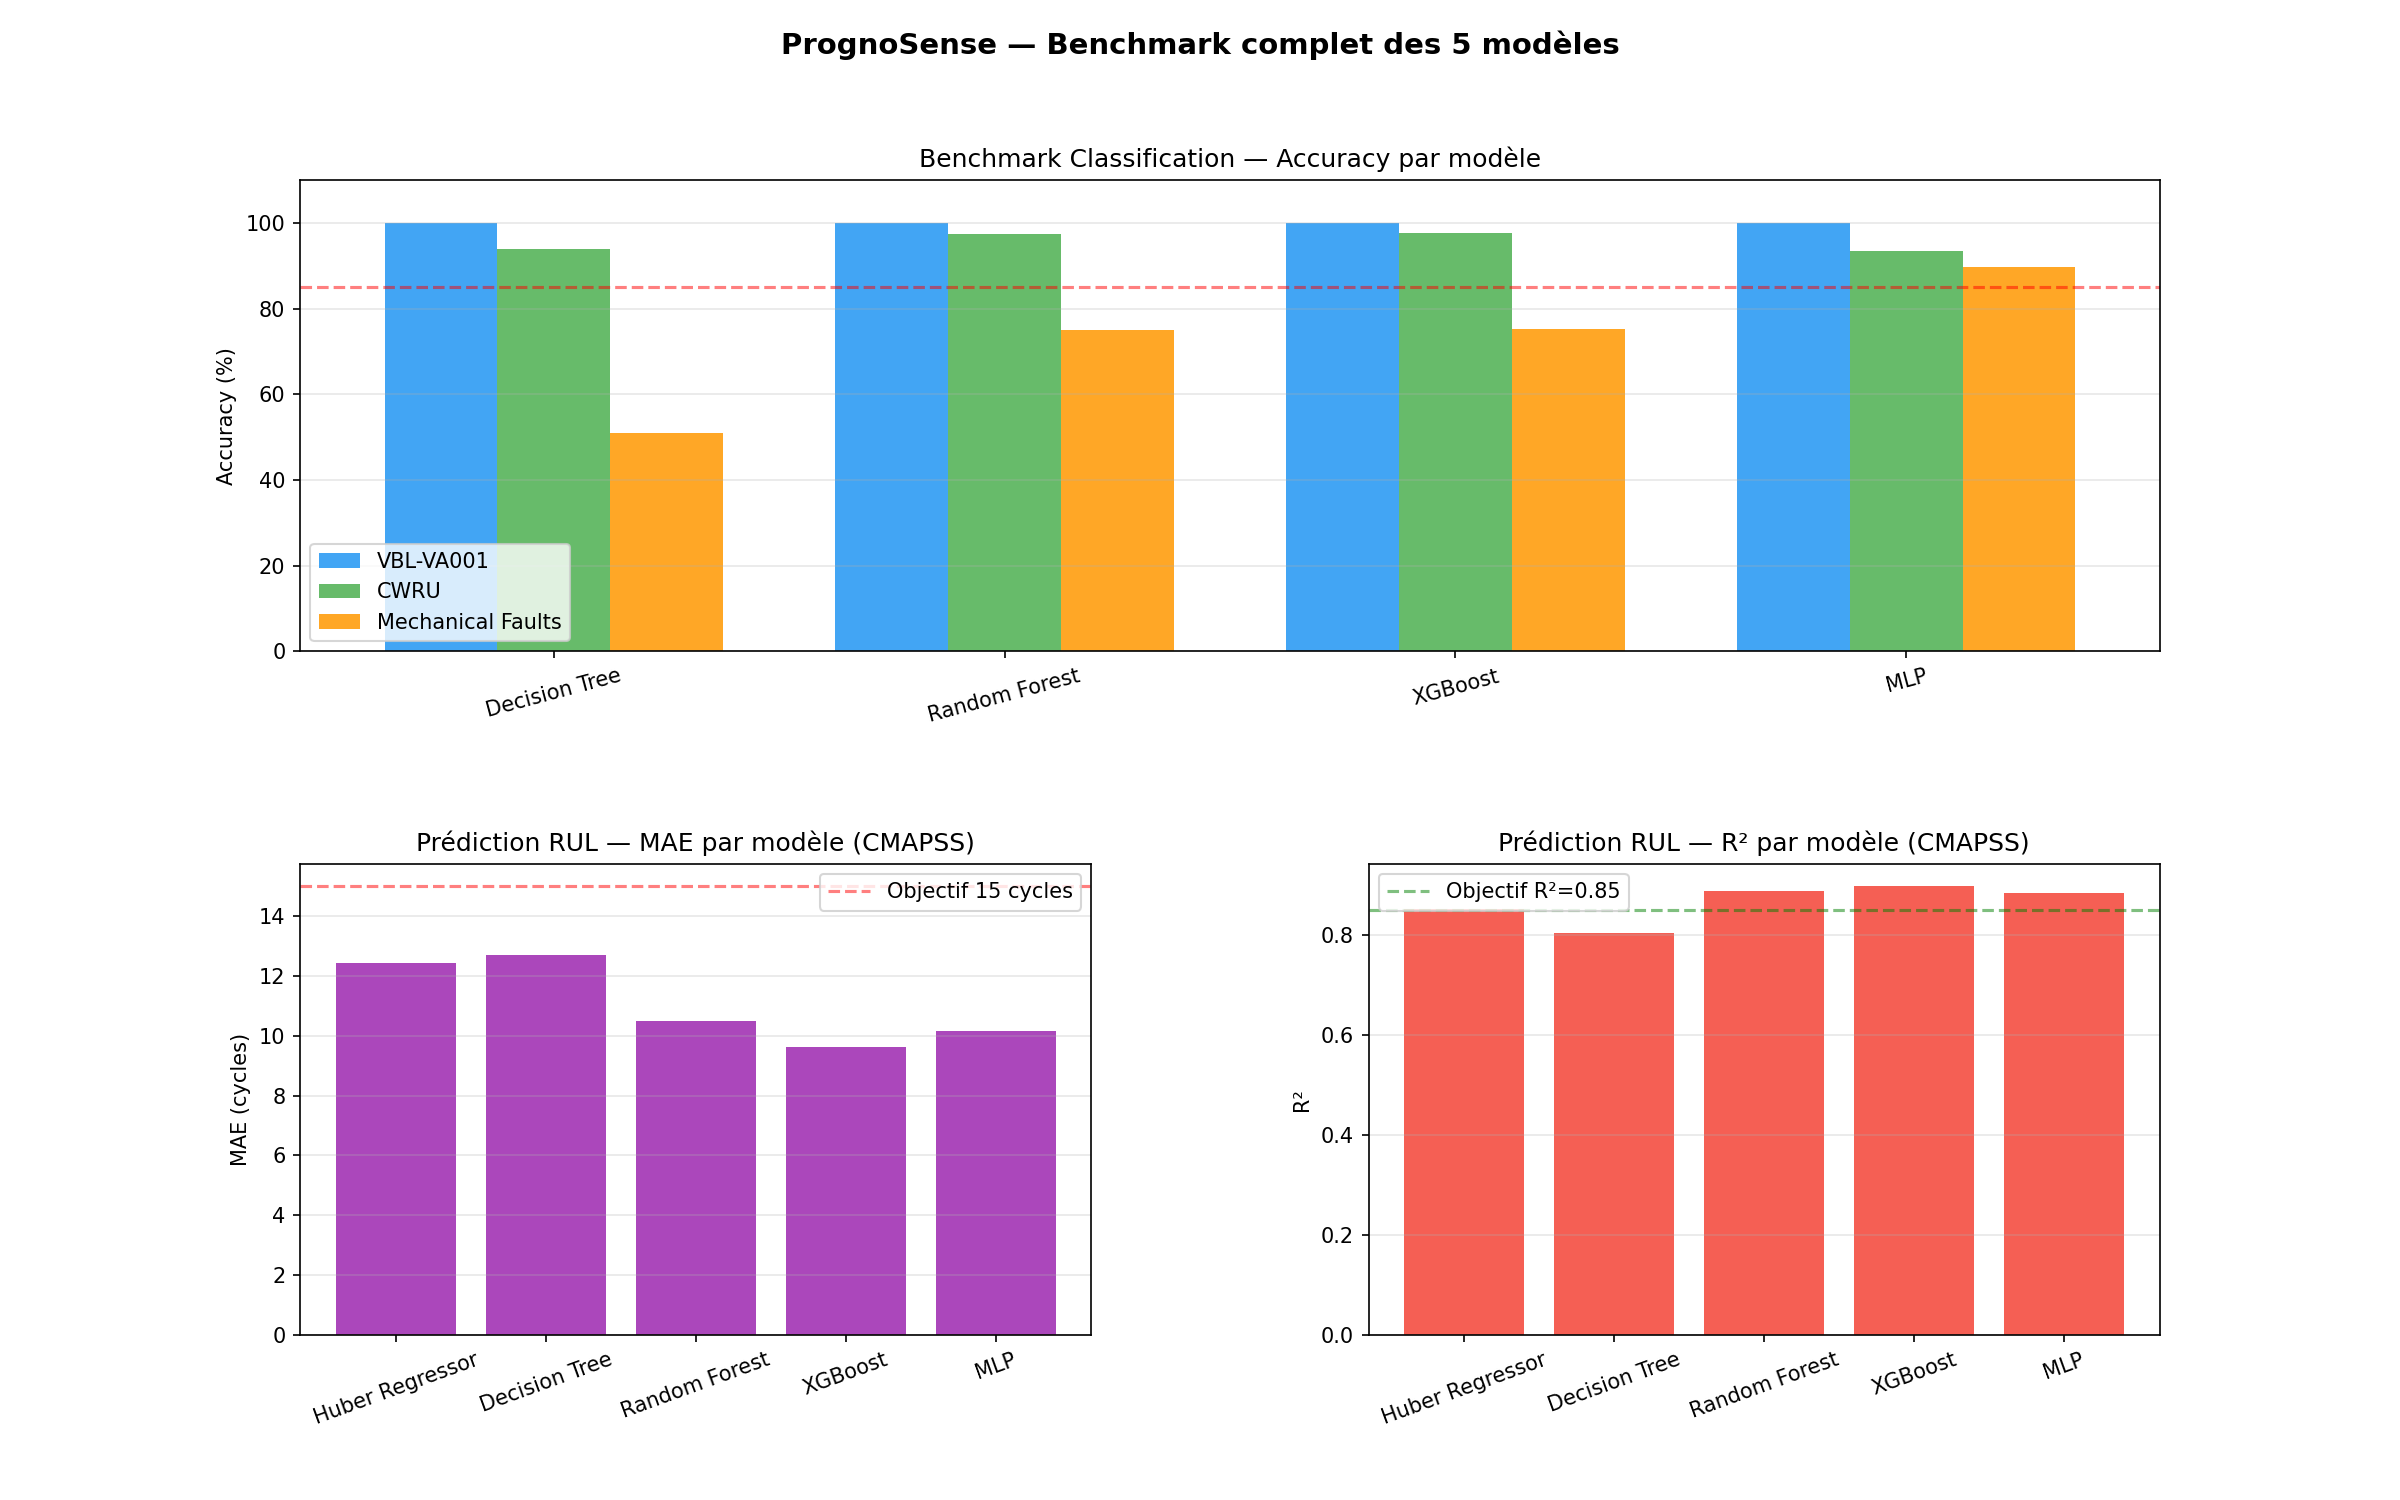
\includegraphics[width=0.95\textwidth]{benchmark_complet.png}
\caption{Synthèse du benchmark des cinq modèles (accuracy en classification, MAE et
$R^2$ en régression RUL).}
\label{fig:bench}
\end{figure}

\subsection{Analyse par dataset}
\textbf{VBL-VA001 (100\,\%).} Les quatre modèles atteignent l'exactitude parfaite. Ce
résultat, loin d'être anodin, valide le pipeline de bout en bout : sur un cas où les classes
sont nettement séparables, aucune erreur n'est introduite par le traitement. Le découpage
par fichier source garantit qu'il ne s'agit pas de sur-apprentissage.

\textbf{CWRU (97{,}6\,\% avec XGBoost).} Sur 10 classes croisant localisation et sévérité,
XGBoost et Random Forest dépassent 97\,\%, démontrant que les features extraites capturent
finement la signature des défauts de roulement et même leur \emph{intensité}. Le Decision
Tree (93{,}9\,\%) et le MLP (93{,}5\,\%) restent honorables. La matrice de confusion
(figure~\ref{fig:cm_cwru}) montre que les rares confusions surviennent entre sévérités
voisines d'un même défaut --- une erreur \emph{bénigne} industriellement.

\textbf{Mechanical Faults (89{,}6\,\% avec le MLP).} C'est le cas le plus instructif. Le
Decision Tree s'effondre (50{,}9\,\%), les méthodes d'arbres plafonnent à 75\,\%, mais le
\textbf{MLP atteint 89{,}6\,\%}. Cette inversion de hiérarchie s'explique : avec 132 features
issues de 4 capteurs et des frontières de décision fortement non linéaires, le réseau de
neurones exploite les interactions entre descripteurs que les arbres peinent à capturer.
\emph{C'est précisément ce que justifie le benchmark} : aucun modèle n'est universellement
supérieur, le choix doit être fait par dataset.

\begin{figure}[h]
\centering
\begin{subfigure}{0.48\textwidth}
  \centering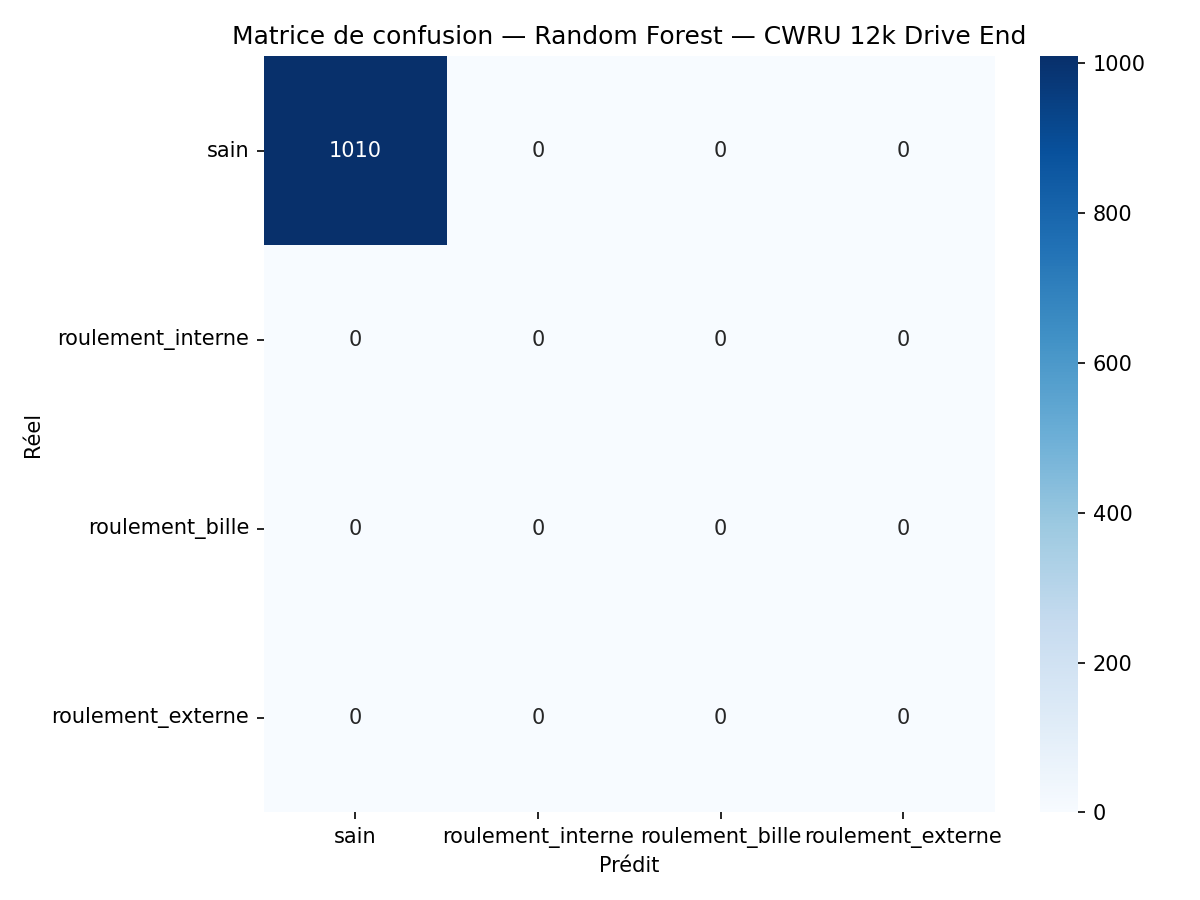
\includegraphics[width=\textwidth]{confusion_matrix_cwru.png}
  \caption{CWRU (10 classes), XGBoost.}
  \label{fig:cm_cwru}
\end{subfigure}\hfill
\begin{subfigure}{0.48\textwidth}
  \centering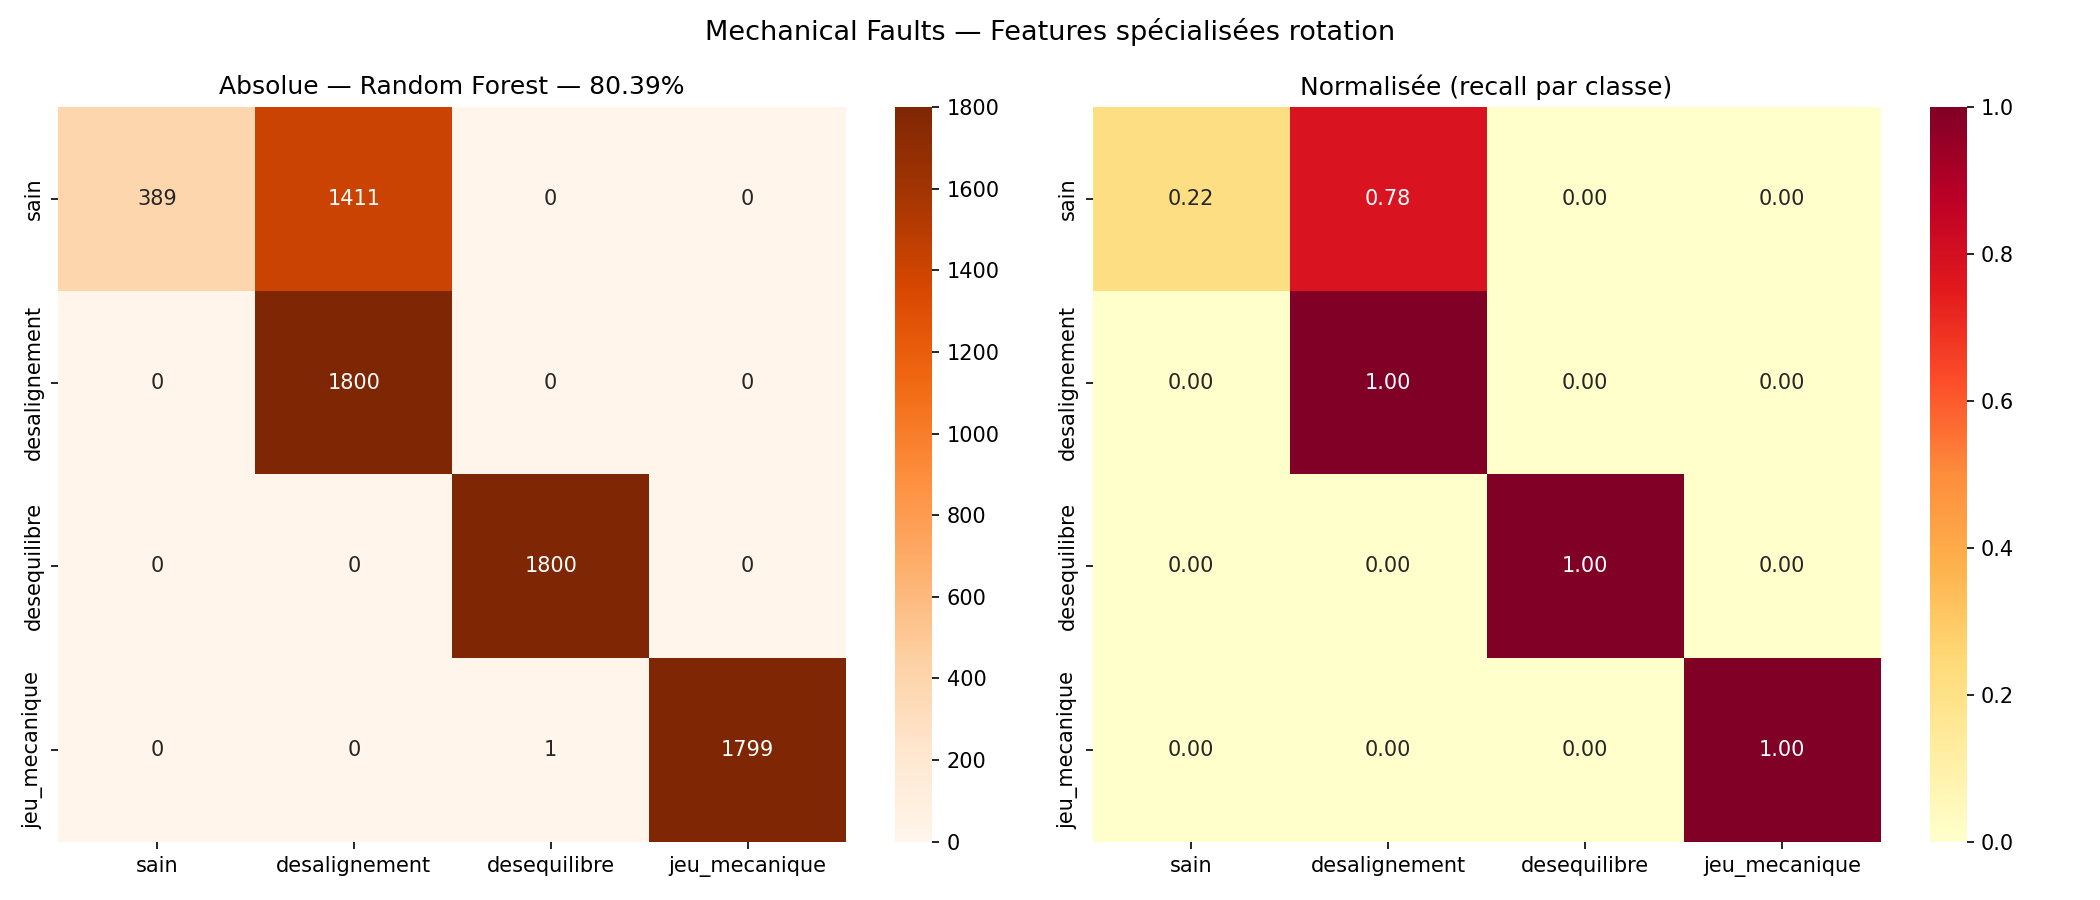
\includegraphics[width=\textwidth]{confusion_matrix_mf_v2.png}
  \caption{Mechanical Faults (4 classes), MLP.}
  \label{fig:cm_mf}
\end{subfigure}
\caption{Matrices de confusion (jeu de test, découpage par fichier source).}
\label{fig:cm}
\end{figure}

\section{Résultats de régression (RUL)}
Le tableau~\ref{tab:regress} présente les résultats de pronostic sur CMAPSS FD001. La
figure~\ref{fig:rul} compare la RUL prédite à la RUL réelle.

\begin{table}[h]
\centering\small
\caption{Benchmark régression RUL --- CMAPSS FD001 (résultats réels).}
\label{tab:regress}
\begin{tabular}{l c c c c c}
\toprule
Modèle & MAE (cycles) & RMSE (cycles) & $R^2$ & Score NASA & Train (s) \\
\midrule
Huber Regressor & 12{,}44 & 16{,}02 & 0{,}853 & 14\,691 & 14{,}6 \\
Decision Tree   & 12{,}70 & 18{,}53 & 0{,}804 & 45\,826 & 2{,}0 \\
Random Forest   & 10{,}50 & 14{,}00 & 0{,}888 & 13\,255 & 69{,}8 \\
\textbf{XGBoost} & \textbf{9{,}61} & \textbf{13{,}35} & \textbf{0{,}898} & \textbf{12\,249} & 18{,}9 \\
MLP             & 10{,}15 & 14{,}22 & 0{,}884 & 13\,098 & 60{,}5 \\
\bottomrule
\end{tabular}
\end{table}

XGBoost domine sur \emph{toutes} les métriques : une \textbf{erreur absolue moyenne de
9{,}61 cycles} et un coefficient de détermination $R^2 = 0{,}90$ signifient que le modèle
explique 90\,\% de la variance de la durée de vie restante, avec une erreur typique
inférieure à 10 cycles. Le Decision Tree, malgré un MAE proche, obtient un score NASA
catastrophique (45\,826 contre 12\,249), révélant qu'il commet des sur-estimations
dangereuses que la métrique asymétrique pénalise --- illustration de l'importance de choisir
la bonne métrique en maintenance.

\begin{figure}[h]
\centering
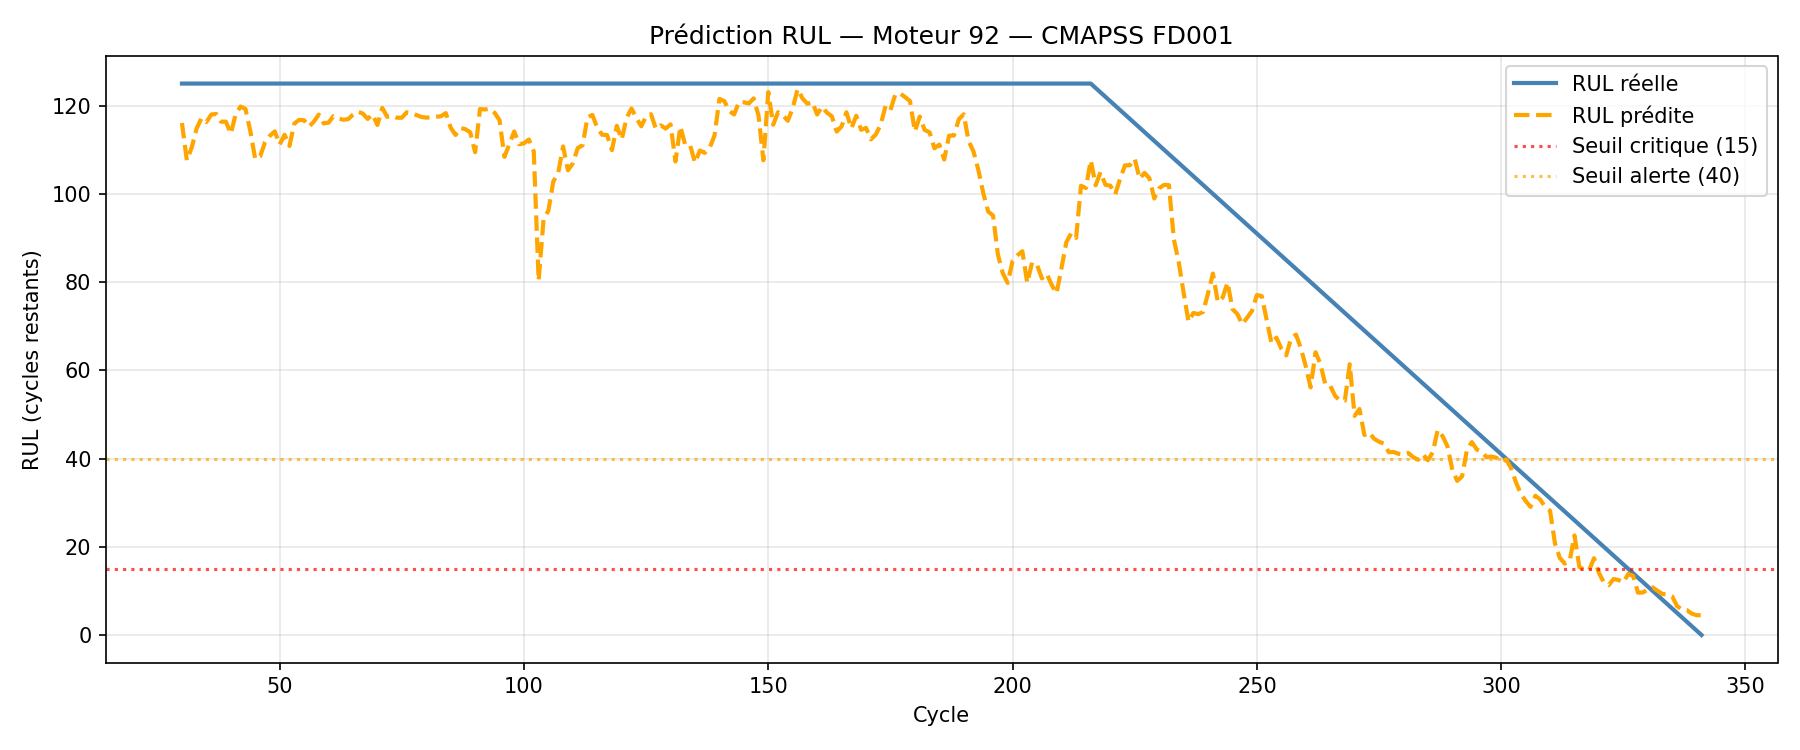
\includegraphics[width=0.8\textwidth]{rul_prediction_cmapss.png}
\caption{RUL prédite vs réelle (CMAPSS), modèle XGBoost.}
\label{fig:rul}
\end{figure}

\section{Cas particulier : CNN 1D pour les engrenages (MCC5-THU)}
Le dataset d'engrenages MCC5-THU est traité différemment : plutôt qu'une extraction
manuelle de features, un \textbf{réseau de neurones convolutif 1D} (\texttt{GearFaultCNN},
PyTorch) apprend directement les motifs pertinents à partir du signal tri-axial. Cette
approche \emph{end-to-end} est adaptée aux signatures d'engrenage (fréquence d'engrènement
GMF et bandes latérales) difficiles à résumer par des descripteurs génériques. Le CNN
classe les huit modes de défaut, y compris les défauts \emph{mixtes}.

\begin{figure}[h]
\centering
\begin{subfigure}{0.46\textwidth}
  \centering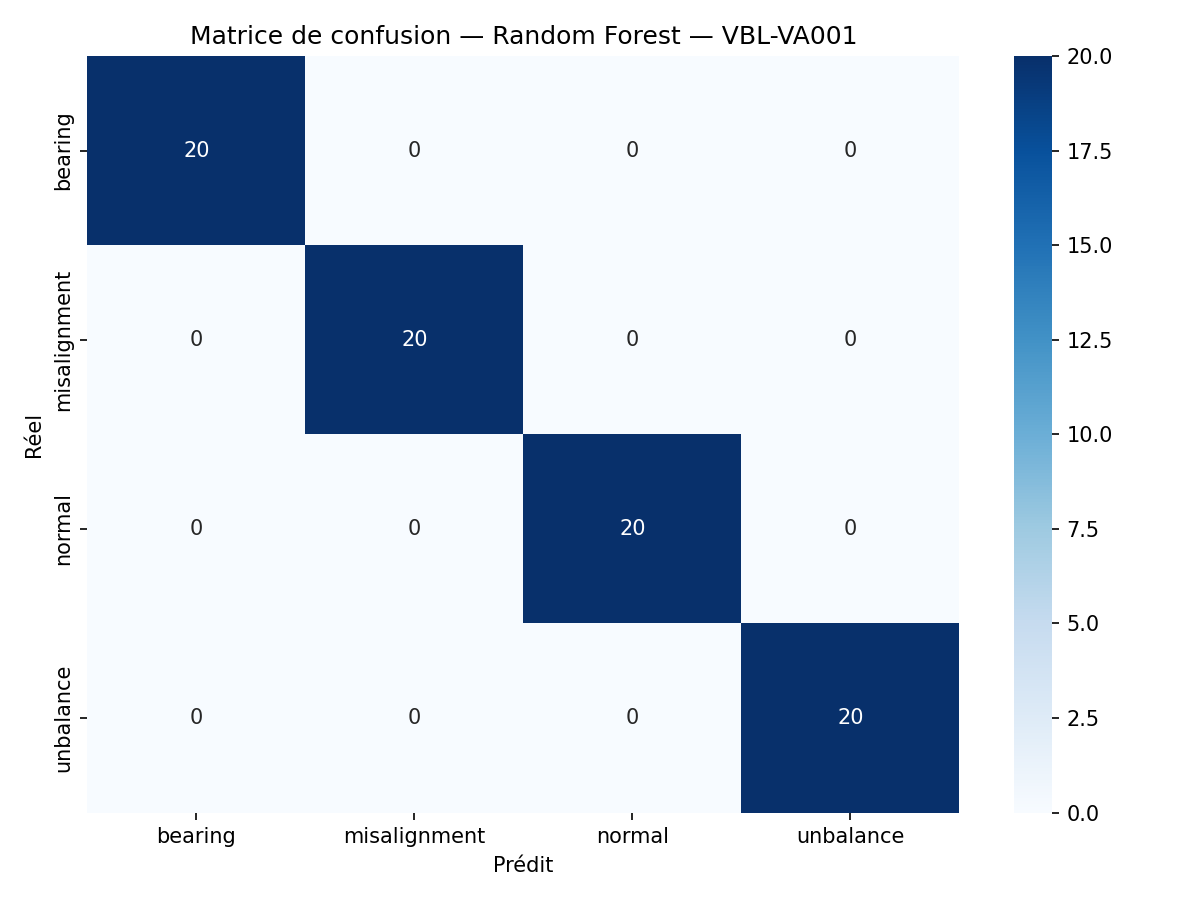
\includegraphics[width=\textwidth]{confusion_matrix_vbl.png}
  \caption{VBL-VA001 (4 classes) --- séparation parfaite.}
  \label{fig:cm_vbl}
\end{subfigure}\hfill
\begin{subfigure}{0.46\textwidth}
  \centering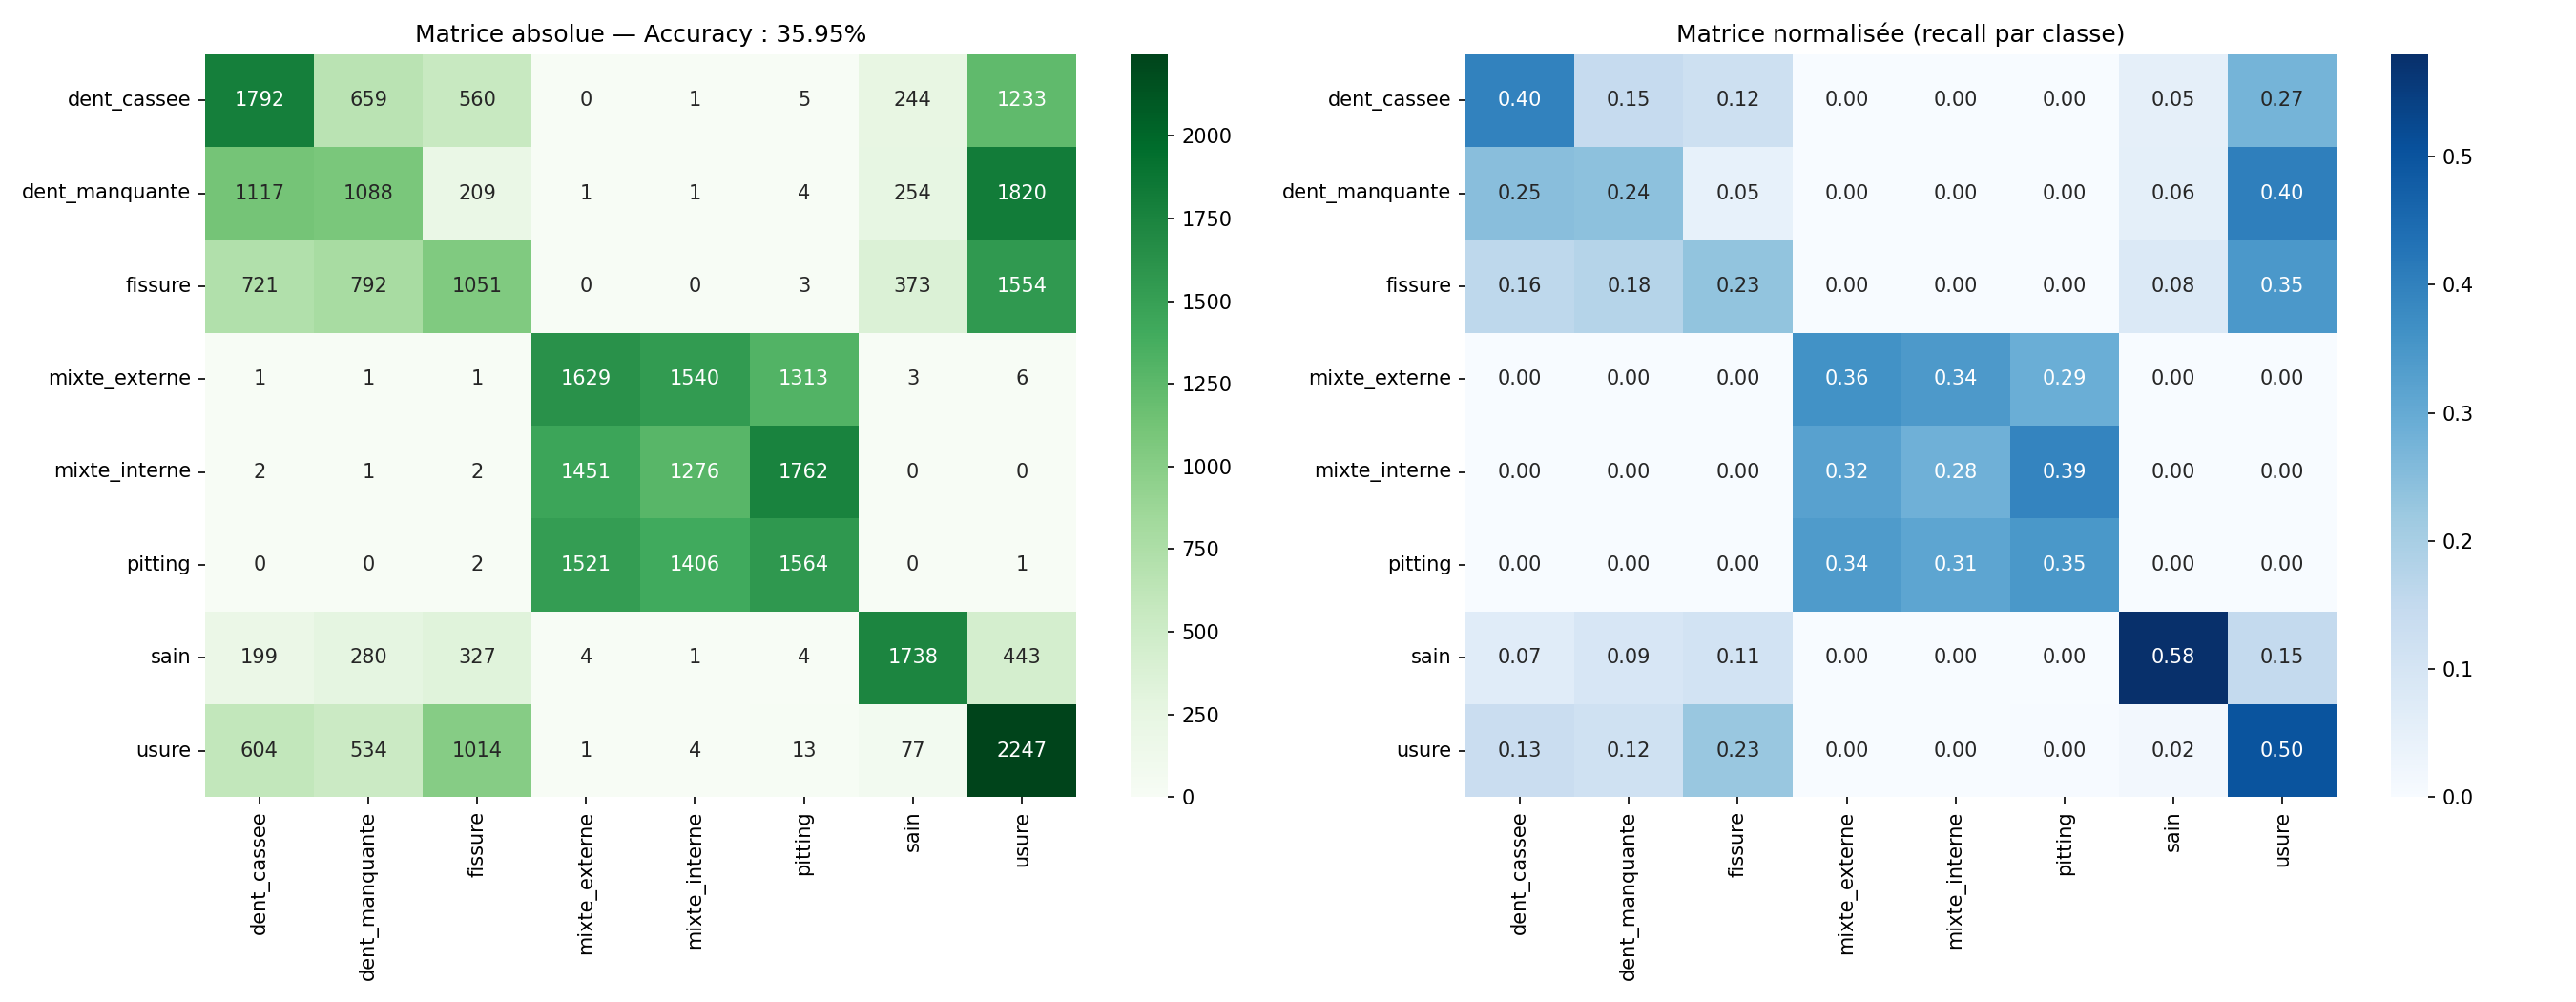
\includegraphics[width=\textwidth]{confusion_matrix_mcc5_v3.png}
  \caption{MCC5-THU (engrenages, 8 classes) --- CNN 1D.}
  \label{fig:cm_mcc5}
\end{subfigure}
\caption{Matrices de confusion complémentaires.}
\label{fig:cm2}
\end{figure}

\section{Sélection des modèles actifs}
À l'issue du benchmark, les modèles finaux sont entraînés sur \textbf{100\,\% des données}
et déployés. Le tableau~\ref{tab:actifs} récapitule les choix, fondés sur les performances
réelles. La plateforme conserve néanmoins \emph{tous} les modèles : l'interface IA Lab
permet de basculer le modèle actif d'un dataset à chaud, sans interruption.

\begin{table}[h]
\centering\small
\caption{Modèles déployés par défaut et justification.}
\label{tab:actifs}
\begin{tabular}{>{\bfseries}l l l}
\toprule
Dataset & Modèle actif & Justification \\
\midrule
VBL-VA001 & XGBoost & 100\,\% + inférence rapide \\
CWRU & XGBoost & meilleure exactitude (97{,}6\,\%) \\
Mechanical Faults & MLP & nettement supérieur (89{,}6\,\% vs 75\,\%) \\
CMAPSS & XGBoost & meilleur MAE/RMSE/$R^2$/NASA \\
MCC5-THU & CNN 1D & apprentissage end-to-end des engrenages \\
\bottomrule
\end{tabular}
\end{table}

\chapter{Détection d'anomalies non supervisée}
\label{chap:anomalie}

\section{Motivation}
Les classifieurs supervisés (chapitre~\ref{chap:bench}) ne reconnaissent que les défauts
\emph{vus à l'entraînement}. Or une part importante des défaillances industrielles relève de
modes rares ou imprévus. Pour combler cet angle mort, PrognoSense intègre une couche de
détection d'anomalies \textbf{non supervisée}, entraînée uniquement sur des données saines :
tout écart au régime normal est signalé, qu'il corresponde ou non à un défaut catalogué.

\section{Auto-encodeur}
\subsection{Architecture}
L'auto-encodeur (PyTorch) est un réseau symétrique encodeur-décodeur qui apprend à
\emph{reconstruire} les vecteurs de features sains via un goulot d'étranglement de dimension
16 (espace latent). L'encodeur enchaîne des couches $d \to 256 \to 128 \to 64 \to 16$ avec
normalisation par lots (\emph{BatchNorm}), activations ReLU et \emph{Dropout} (0{,}2) ; le
décodeur est le miroir. La dimension d'entrée $d$ s'adapte au dataset (45 pour VBL, 15 pour
CWRU, 132 pour MF, 126 pour CMAPSS).

\subsection{Principe de détection}
Entraîné à minimiser l'erreur quadratique de reconstruction sur les seules données saines,
l'auto-encodeur reconstruit fidèlement un signal normal mais échoue sur un signal anormal.
L'\textbf{erreur de reconstruction}~\eqref{eq:recon} sert donc de score d'anomalie :
\begin{equation}
\varepsilon(x) = \tfrac{1}{d}\,\lVert x - \hat{x} \rVert_2^2
\label{eq:recon}
\end{equation}
Le \textbf{seuil de décision} est fixé au \textbf{95\textsuperscript{e} percentile} des
erreurs de reconstruction sur les données d'entraînement : 95\,\% des données saines sont
ainsi correctement reconnues comme normales. Les seuils réels obtenus sont reportés au
tableau~\ref{tab:ae}. Le score est ensuite normalisé sur $[0,100]$ par rapport aux
percentiles P5--P99 des erreurs d'entraînement.

\begin{table}[h]
\centering\small
\caption{Auto-encodeurs entraînés : dimension d'entrée et seuil (P95).}
\label{tab:ae}
\begin{tabular}{>{\bfseries}l c c}
\toprule
Dataset & Dimension d'entrée & Seuil P95 (erreur) \\
\midrule
VBL    & 45  & 0{,}1049 \\
CWRU   & 15  & 0{,}0493 \\
MF     & 132 & 0{,}5693 \\
CMAPSS & 126 & 0{,}3161 \\
\bottomrule
\end{tabular}
\end{table}

\begin{figure}[h]
\centering
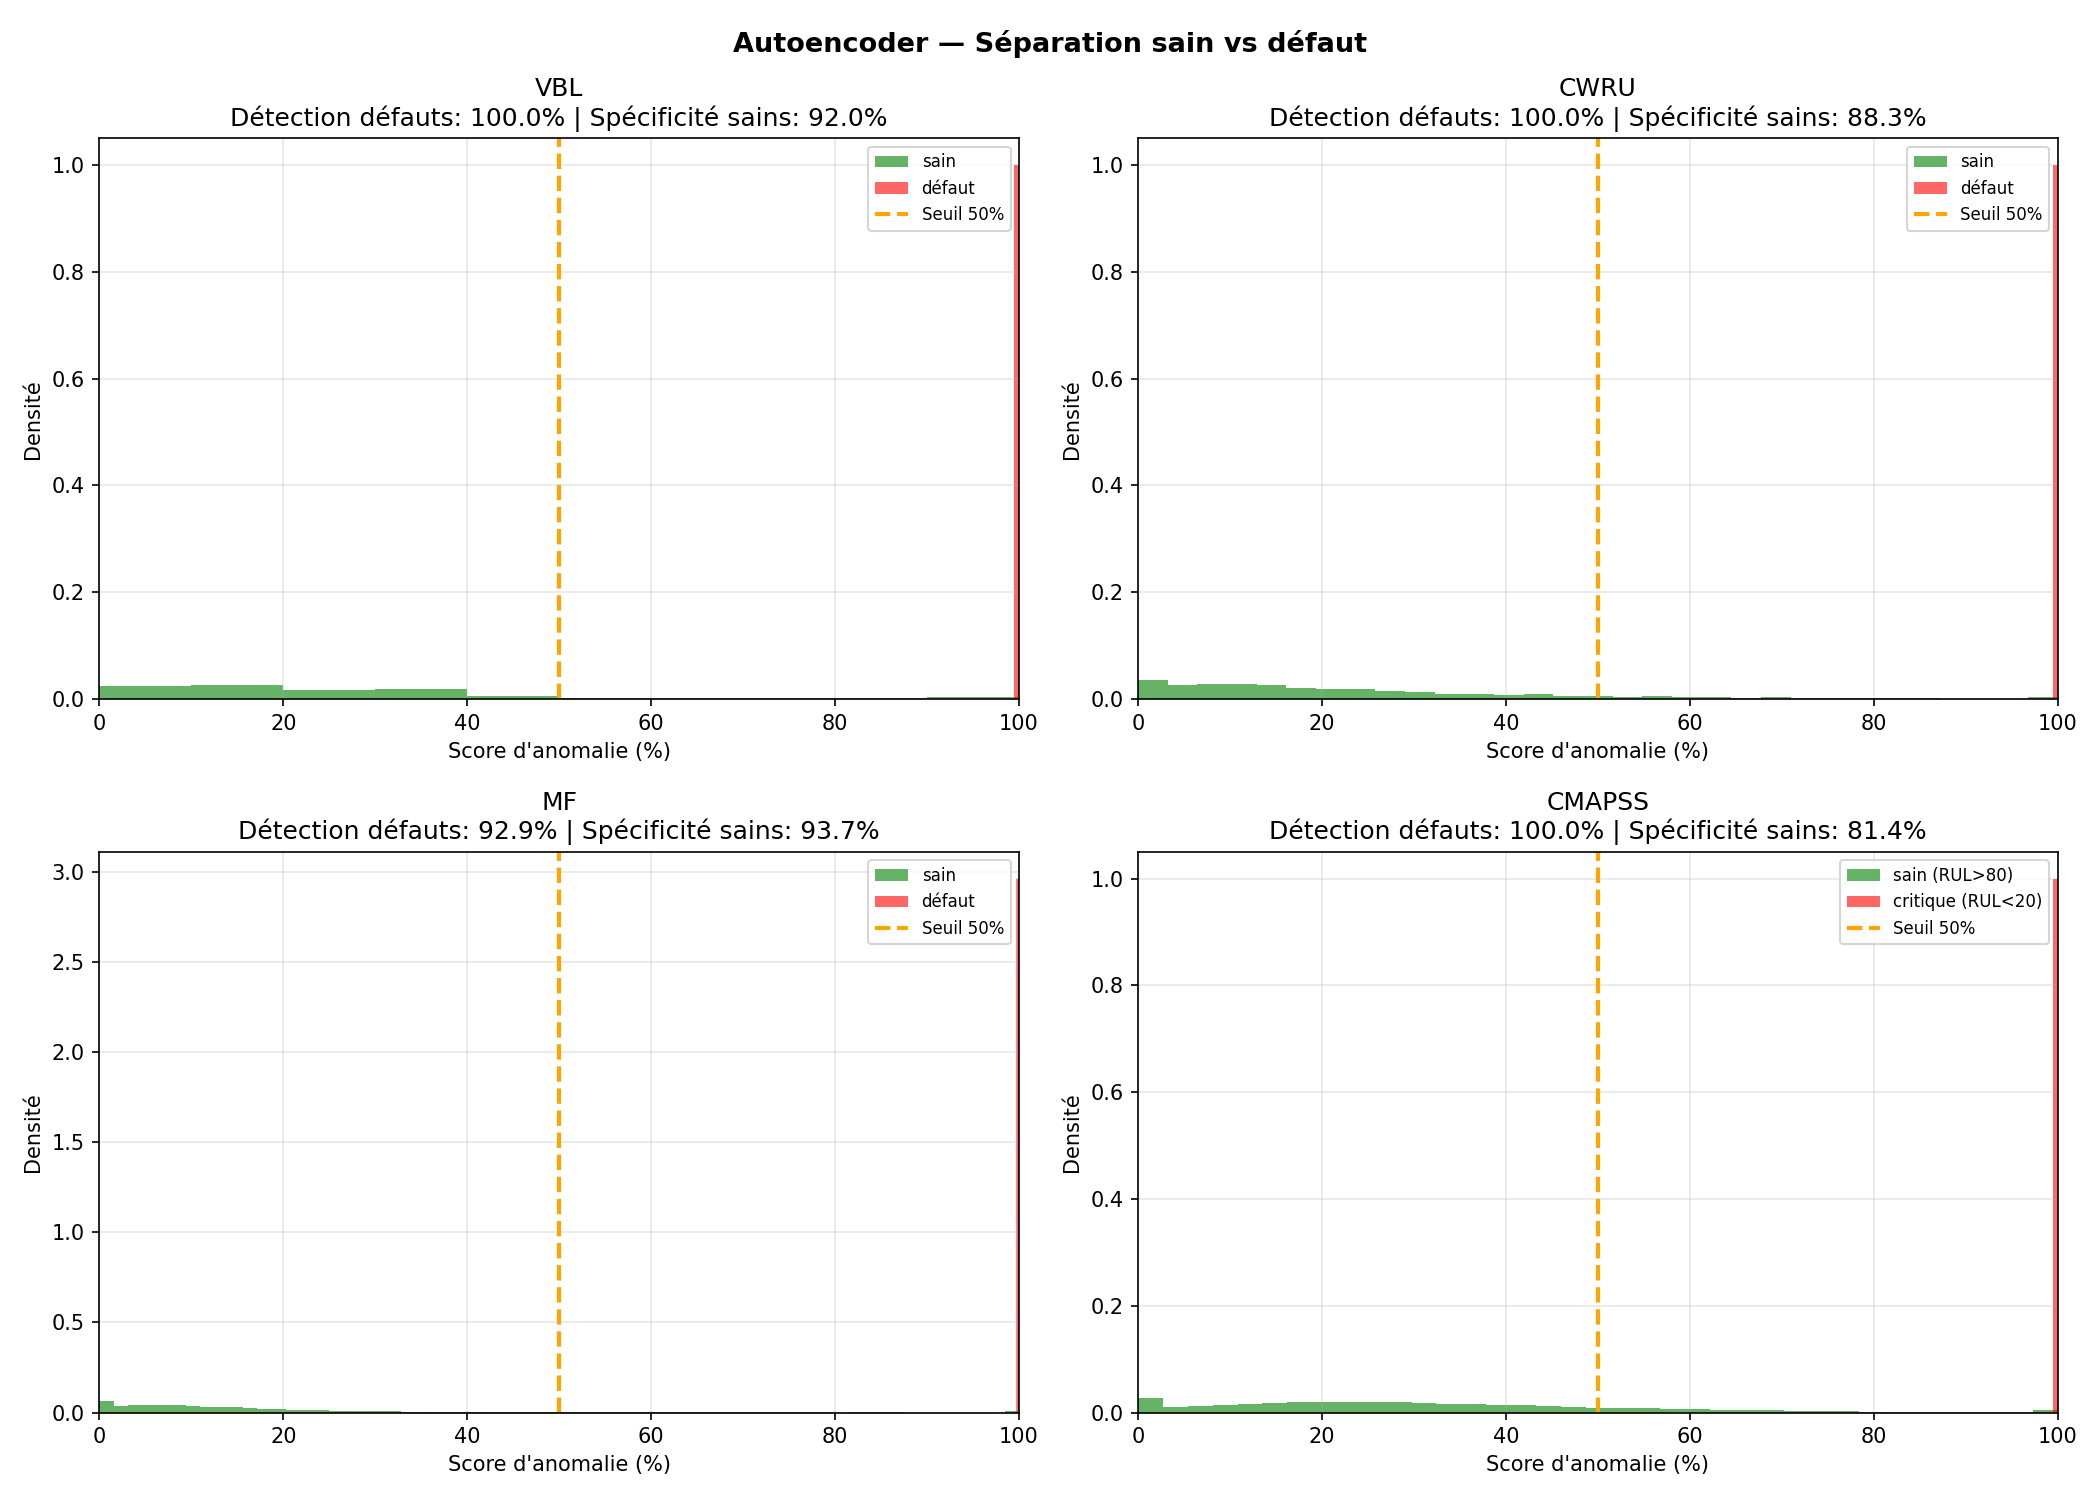
\includegraphics[width=0.85\textwidth]{autoencoder_validation.png}
\caption{Validation de l'auto-encodeur : distribution des erreurs de reconstruction
sain vs défaut, et seuil de décision.}
\label{fig:ae}
\end{figure}

\section{Ensemble de détecteurs (vote par consensus)}
Pour fiabiliser la décision et \textbf{réduire les fausses alarmes}, un second dispositif
combine trois détecteurs d'anomalie aux biais complémentaires :
\begin{itemize}[leftmargin=1.5em]
  \item \textbf{Isolation Forest} : isole les points rares par partitionnement aléatoire,
        efficace en haute dimension ;
  \item \textbf{Local Outlier Factor} : compare la densité locale d'un point à celle de ses
        voisins ;
  \item \textbf{Elliptic Envelope} : suppose une distribution gaussienne et détecte les
        déviations de covariance.
\end{itemize}
Une anomalie n'est \textbf{confirmée que par vote majoritaire} : au moins deux des trois
détecteurs doivent s'accorder. Ce consensus diminue fortement le risque de fausse alerte
isolée. Pour produire des scores stables même sur un seul échantillon, chaque détecteur est
calibré contre une \textbf{référence de normalité} (percentiles P1--P99 de sa fonction de
décision sur les données saines), plutôt que normalisé au sein du lot courant.

\section{Apprentissage du baseline propre à chaque machine}
La détection non supervisée a été poussée plus loin avec le module \texttt{MachineBaseline}.
Plutôt que de comparer une machine à un dataset public générique, la plateforme apprend la
\textbf{signature saine spécifique de chaque machine} (statistiques multivariées : moyenne
et écart-type de chaque feature sur une fenêtre d'apprentissage). L'anomalie est alors
mesurée relativement à \emph{cette} machine :
\begin{equation}
z_i = \left|\frac{x_i - \mu_i}{\sigma_i}\right|, \qquad
s = \min\!\Big(100,\ 60\cdot \tfrac{1}{d}\textstyle\sum_i \mathbb{1}[z_i>3]
   + 40\cdot \min(1, \bar{z}/5)\Big)
\end{equation}
Ce score combine la proportion de features fortement déviantes ($z>3$) et l'ampleur moyenne
de la déviation. Validation : sur un signal sain le score reste $\approx 5\,\%$, sur un
signal dégradé il atteint $\approx 96\,\%$, avec identification des \emph{features
contributrices} (explicabilité). Cette approche --- apprendre le \og normal \fg{} de chaque
équipement sans aucun historique de panne --- est celle des solutions industrielles de
pointe, et constitue un apport majeur du projet (chapitre~\ref{chap:indus}).

\chapter{Architecture backend (FastAPI)}
\label{chap:backend}

\section{Organisation}
Le backend est structuré en \textbf{routeurs spécialisés} (un par domaine fonctionnel),
montés sous le préfixe \texttt{/api}. Au démarrage, l'application initialise la base de
données, charge l'ensemble des modèles via le \texttt{ModelRegistry}, instancie la flotte
de démonstration et active les connecteurs industriels éventuels. Le
tableau~\ref{tab:routes} recense les principaux groupes de routes.

\begin{table}[h]
\centering\small
\caption{Principaux groupes de routes de l'API.}
\label{tab:routes}
\begin{tabular}{>{\bfseries}l p{9.5cm}}
\toprule
Domaine & Routes principales \\
\midrule
Prédiction & \texttt{/predict}, \texttt{/model/select}, \texttt{/model/active/\{ds\}},
             \texttt{/model/versions/\{ds\}/\{m\}}, \texttt{/model/rollback} \\
Flotte / santé & \texttt{/fleet}, \texttt{/machine/\{id\}}, \texttt{/machine/\{id\}/history} \\
Simulation & \texttt{/ws/simulation} (WebSocket), \texttt{/simulation/units} \\
Analyse spectrale & \texttt{/signal/indicators}, \texttt{/signal/spectrum},
             \texttt{/signal/diagnose}, \texttt{/signal/iso-severity}, \texttt{/bearing/frequencies} \\
Ingestion & \texttt{/ingest/signal}, \texttt{/ingest/baseline/\{finalize,reset,status\}}, \texttt{/replay/\{ds\}/\{idx\}} \\
Anomalie & \texttt{/anomaly/ensemble/\{ds\}}, \texttt{/anomaly/ensemble/demo/\{ds\}} \\
KPIs / analytics & \texttt{/kpi/real/\{id\}}, \texttt{/kpi/roi/\{id\}},
             \texttt{/analytics/prediction-accuracy/\{id\}}, \texttt{/analytics/false-alarm-rate} \\
GMAO & \texttt{/workorder(s)}, \texttt{/maintenance/event} \\
Confiance & \texttt{/drift/status}, \texttt{/audit/recent}, \texttt{/explain/shap},
             \texttt{/explain/calibration/\{ds\}} \\
Copilot & \texttt{/copilot/chat}, \texttt{/copilot/report/\{id\}} \\
Sécurité & \texttt{/auth/register}, \texttt{/auth/login}, \texttt{/auth/me} \\
Retrain & \texttt{/retrain/start}, \texttt{/retrain/demo}, \texttt{/retrain/status} \\
\bottomrule
\end{tabular}
\end{table}

\section{Le registre de modèles}
Le \texttt{ModelRegistry} est la pièce maîtresse du backend. Il centralise le chargement
(registre benchmark, auto-encodeurs, CNN, MLP spécialisés), la gestion du modèle actif par
dataset (persistée en JSON), l'inférence unifiée, le réentraînement asynchrone et le
versioning. L'interface de prédiction unifiée applique systématiquement la même logique :
sélection du modèle actif (ou imposé), normalisation conditionnelle des entrées (uniquement
pour le MLP et le Huber, sensibles à l'échelle), exécution du monitoring de dérive en
parallèle, puis production d'un résultat au format homogène. Pour une tâche de régression
(CMAPSS), la sortie est la RUL moyenne plafonnée à 125 cycles ; pour une tâche de
classification, elle comprend le label décodé (via le \emph{LabelEncoder} du dataset) et un
niveau de confiance dérivé des probabilités. Ce format uniforme, indépendant du modèle
sous-jacent, simplifie la consommation côté client et l'intégration de nouveaux modèles.

\section{La simulation temps réel}
Le c\oe ur dynamique de la plateforme est le WebSocket de simulation. À chaque cycle, pour
la machine surveillée, le serveur : (i) sélectionne la fenêtre de données réelle suivante,
(ii) exécute la prédiction supervisée et le score d'anomalie, (iii) calcule l'indice de
santé lissé, (iv) reconstruit un signal exploitable pour l'affichage spectral, (v) met à
jour le \texttt{HealthTracker} (historique, tendance, alertes) et (vi) diffuse un message
JSON complet. Toutes les cinq itérations, l'événement est consigné dans le journal d'audit
et persisté en base. Un \texttt{ConnectionManager} isole l'état de chaque client (machine,
dataset, vitesse), permettant la surveillance simultanée de plusieurs machines.

\section{Sécurité et persistance}
L'\textbf{authentification} repose sur des jetons \textbf{JWT} signés (HS256, expiration
configurable) et des mots de passe hachés en \textbf{bcrypt}. Deux rôles sont gérés :
\texttt{admin} (réentraînement, injection de défauts, rollback) et \texttt{user}
(consultation). La \textbf{persistance} s'appuie sur SQLAlchemy : les modèles
\texttt{MachineState}, \texttt{Alert}, \texttt{DiagnosticLog}, \texttt{ModelMetadata},
\texttt{User}, \texttt{MaintenanceEvent}, \texttt{ModelVersion}, \texttt{WorkOrder} et
\texttt{AlertVerdict} couvrent l'ensemble du domaine. Le mode \textbf{WAL} de SQLite autorise
lectures et écriture concurrentes, indispensable à la coexistence de la boucle de simulation,
des écritures d'événements et du versioning.

\section{Validation des entrées}
Toutes les entrées sont validées par des schémas \textbf{Pydantic} (longueur minimale de
signal, positivité des fréquences, géométrie de roulement cohérente), ce qui sécurise l'API
contre les données malformées et documente automatiquement le contrat d'interface via
Swagger (\texttt{/docs}).

\chapter{Interface utilisateur (React)}
\label{chap:frontend}

\section{Principes d'interface}
Le frontend, développé en \textbf{React} avec le bundler \textbf{Vite}, vise un usage par
des ingénieurs de maintenance, non par des spécialistes de la donnée. Il privilégie la
lisibilité immédiate (codes couleur sémantiques vert/jaune/orange/rouge), l'information en
temps réel (WebSocket) et des graphiques interactifs (\textbf{Recharts}). L'accès est
protégé par une page de connexion ; un intercepteur ajoute automatiquement le jeton JWT à
chaque requête et gère son expiration. Un \emph{error boundary} global garantit qu'une
erreur de rendu d'une page n'interrompt jamais toute l'application.

\section{Les pages fonctionnelles}
\subsection{Connexion}
Authentification par e-mail et mot de passe, avec gestion des rôles. La session est
conservée localement et expire automatiquement.

\subsection{Vue Globale}
Tableau de bord de la flotte : chaque machine est présentée par une carte affichant son
indice de santé (jauge), sa RUL estimée, sa tendance et son statut. Les KPIs agrégés
(machines saines, en alerte, critiques, indice moyen) sont en tête. Un clic sur une machine
déclenche sa surveillance temps réel et ouvre un panneau détaillé (indice de santé, RUL,
score d'anomalie, défaut détecté avec niveau de confiance).

\subsection{Monitoring}
Surveillance vibratoire en direct : forme d'onde, spectre et indicateurs (RMS, kurtosis,
crête) défilent en temps réel via le WebSocket, avec contrôles de lecture (play/pause,
vitesse) et sélection de la machine.

\subsection{IA Lab}
Centre d'analyse des modèles, organisé en onglets : \emph{Classification} et
\emph{Régression RUL} (graphiques et tableaux du benchmark), \emph{Fiabilité \& Drift}
(score de dérive par dataset, carte d'ensemble d'anomalie), \emph{Explicabilité SHAP}
(importance des indicateurs), \emph{Calibration} (diagramme de fiabilité, ECE) et
\emph{Versions Modèle} (historique des versions et \textbf{retour arrière} en un clic).
L'utilisateur peut y \textbf{basculer le modèle actif} d'un dataset à chaud.

\subsection{Pronostic \& RUL}
Visualisation de la trajectoire de dégradation (courbe d'indice de santé avec seuils
70/40/20\,\%) et compte à rebours de la durée de vie restante, avec comparaison RUL prédite
vs réelle pour les turbomoteurs CMAPSS.

\subsection{Maintenance}
Page opérationnelle centrale, enrichie de plusieurs panneaux : le \emph{journal d'alertes},
le \emph{copilot} conversationnel, le \emph{diagnostic par spectre externe} (import CSV/JSON),
la \emph{saisie d'événements de maintenance}, le panneau \emph{KPIs réels \& efficacité
prédictive} (MTBF, MTTR, disponibilité, ROI, précision/rappel/lead-time), le panneau
\emph{Ordres de travail} (boucle GMAO) et le \emph{réentraînement} piloté.

\subsection{Audit Trail}
Journal de traçabilité : chaque décision de l'IA et chaque alerte y est horodatée
(prédiction, machine, confiance), avec compteurs et filtres. Cette page matérialise
l'exigence \og rien n'est une boîte noire \fg.

\subsection{Configuration}
Réglage des seuils (anomalie, sévérité), des paramètres de roulement et des préférences de
la plateforme.

\section{Communication temps réel}
Le hook \texttt{useSimulationWS} encapsule la connexion WebSocket : ouverture, envoi des
commandes (play, pause, set\_machine), réception et bufferisation de l'historique, et
surtout \textbf{reconnexion automatique à back-off exponentiel} en cas de coupure. Les pages
consomment ce hook pour afficher des données vivantes sans recharger.

\section{Composants réutilisables}
Des composants d'interface (\texttt{HealthGauge} pour la jauge de santé, \texttt{MetricCard}
pour les indicateurs) assurent la cohérence visuelle. La charte graphique (fond sombre,
accents cyan/vert/ambre) a inspiré les couleurs de ce rapport.

\chapter{Industrialisation : du diagnostic à la solution déployable}
\label{chap:indus}

Ce chapitre regroupe les développements qui font passer PrognoSense d'un démonstrateur
d'analyse à une solution \emph{déployable} et \emph{digne de confiance} sur le terrain.
C'est ici que se concentre la valeur différenciante du projet.

\section{Sévérité normalisée ISO 10816/20816}
La plateforme exprime la sévérité dans le langage des ingénieurs de fiabilité : vitesse
vibratoire efficace en mm/s et zones A/B/C/D par classe de machine (cf.
chapitre~\ref{chap:pipeline}). La zone ISO est calculée à l'ingestion, injectée dans le
diagnostic et affichée dans les ordres de travail. Cela rend chaque diagnostic
\textbf{comparable et défendable}, à la différence d'un indice propriétaire.

\section{Connectivité terrain : du capteur à l'ingestion}
\subsection{Couche d'ingestion universelle}
Le point d'entrée \texttt{POST /api/ingest/signal} accepte une forme d'onde
d'accélération réelle, quelle qu'en soit la source, et la fait traverser tout le pipeline :
extraction d'indicateurs $\rightarrow$ sévérité ISO $\rightarrow$ anomalie vs baseline
machine $\rightarrow$ diagnostic spectral $\rightarrow$ indice de santé $\rightarrow$
persistance et mise à jour de la flotte. Cette abstraction \emph{vendor-agnostic} est ce qui
transforme la plateforme en système connectable au parc existant.

\subsection{OPC-UA}
Un connecteur OPC-UA (bibliothèque \texttt{asyncua}) lit périodiquement un n\oe ud de mesure
sur un serveur OPC-UA --- le protocole standard de l'automatisme industriel. La chaîne
complète a été validée localement à l'aide d'un serveur OPC-UA de démonstration : la machine
virtuelle \texttt{POMPE\_OPCUA} a été correctement lue puis ingérée (états persistés,
baseline créé), prouvant le fonctionnement de bout en bout \emph{capteur} $\rightarrow$
\emph{ingestion}.

\subsection{MQTT}
Un connecteur MQTT (\texttt{paho-mqtt}) souscrit à un topic IIoT et transfère chaque message
vers la même ingestion. Les deux connecteurs sont \emph{activés sur configuration}
(variables d'environnement), sans impact lorsqu'ils ne sont pas utilisés.

\section{Apprentissage du comportement sain par machine}
Comme détaillé au chapitre~\ref{chap:anomalie}, le module \texttt{MachineBaseline} apprend
la signature saine \emph{propre à chaque machine}, sans nécessiter d'historique de pannes.
L'anomalie est mesurée relativement à cette référence : validation à $\approx 5\,\%$ sur un
signal sain et $\approx 96\,\%$ sur un signal dégradé, avec désignation des indicateurs
contributeurs.

\section{Boucle fermée : de l'alerte à l'ordre de travail}
PrognoSense ferme la boucle de maintenance. Lorsqu'une machine atteint un état critique
(zone ISO D ou indice de santé bas), un \textbf{ordre de travail} est créé automatiquement,
avec priorité (P1/P2), machine, défaut et action recommandée, en évitant les doublons (un
seul ordre ouvert par machine). Cet ordre peut être \textbf{poussé vers la GMAO} de
l'entreprise (SAP PM, IBM Maximo, Infor) via un connecteur webhook configurable. L'alerte
devient ainsi une intervention planifiée et tracée. Des notifications par e-mail (SMTP)
complètent le dispositif.

\section{Indicateurs de fiabilité : mesurés, pas estimés}
\subsection{Un choix méthodologique assumé}
Un point central distingue PrognoSense de nombreux prototypes : les indicateurs de fiabilité
ne sont pas \emph{estimés} à partir de la simulation, mais \textbf{mesurés sur l'historique
réel des interventions}, conformément à leur définition normative :
\begin{align}
\text{MTBF} &= \frac{\text{temps de fonctionnement cumulé}}{\text{nombre de pannes réelles}} &
\text{MTTR} &= \frac{\text{temps total de réparation}}{\text{nombre de réparations}} \\
\text{Disponibilité} &= \frac{\text{MTBF}}{\text{MTBF}+\text{MTTR}}\times 100 & & \notag
\end{align}
Un MTBF ne se déduit pas d'un capteur : il se \emph{constate} sur les pannes effectives.
C'est pourquoi la plateforme propose une saisie des événements de maintenance (le \og carnet
de bord \fg) qui alimente ces calculs. Tant qu'aucune donnée n'est saisie, la plateforme
\emph{n'affiche rien} plutôt qu'un chiffre fabriqué --- gage d'honnêteté scientifique.

\subsection{Retour sur investissement}
À partir des interventions, la plateforme estime les arrêts évités et les économies
réalisées (paramètres ajustables : coût horaire de production, durée d'arrêt évitée),
fournissant un argumentaire de ROI exploitable par la direction.

\subsection{Efficacité prédictive et taux de fausses alarmes}
En croisant les alertes émises avec les pannes réelles (fenêtre d'anticipation de 48\,h), la
plateforme calcule la \textbf{précision}, le \textbf{rappel} et le \textbf{lead-time}
(délai d'anticipation moyen). Surtout, un mécanisme de \textbf{validation par l'expert}
(verdict vrai/faux positif sur chaque alerte) permet de mesurer le \emph{vrai} taux de
fausses alarmes --- l'indicateur de confiance le plus exigé par les acheteurs de solutions
PdM. Cette boucle \emph{human-in-the-loop} est, à la connaissance de l'auteur, rarement
présente dans les travaux comparables.

\section{Copilot ancré sur les connaissances (RAG)}
Un assistant conversationnel, propulsé par le modèle de langage \textbf{Mistral}, répond en
langage naturel et dispose du contexte temps réel de la flotte. Il est \textbf{ancré} sur une
base de connaissances (normes ISO, guide des signatures de défaut, interprétation des
indicateurs) via une recherche de similarité \textbf{TF-IDF} (RAG). Ses réponses
\emph{citent les sources documentaires}, ce qui les rend précises et \textbf{traçables}.
Exemple validé : à la question \og quel défaut provoque un pic à 2$\times$ la fréquence de
rotation ?\fg, le copilot répond \og désalignement \fg{} en s'appuyant sur le guide des
défauts, sources à l'appui. Le copilot démocratise ainsi l'expertise d'un analyste vibratoire
auprès des techniciens.

\section{Confiance et gouvernance des modèles}
\subsection{Détection de dérive (concept drift)}
À chaque prédiction, un \texttt{DriftDetector} compare la distribution des données de
production à la distribution d'entraînement par test de \textbf{Kolmogorov-Smirnov}. Une
dérive est signalée lorsque plus de 30\,\% des features testées présentent une p-value
$< 0{,}05$, avec une sévérité critique si $\min(p)<0{,}001$. La plateforme recommande alors
un réentraînement.

\subsection{Calibration des probabilités}
La calibration (isotonique, \texttt{CalibratedClassifierCV}) corrige le biais de confiance :
sans elle, un modèle annonçant \og 94\,\% \fg{} peut n'être correct que dans 75\,\% des cas.
Un diagramme de fiabilité et l'erreur de calibration espérée (ECE) sont calculés ; un modèle
est jugé bien calibré si ECE $< 0{,}05$.

\subsection{Versioning et retour arrière}
Chaque réentraînement crée une \textbf{version} archivée du modèle (métriques, date,
déclencheur). En cas de régression, un \textbf{rollback} en un clic réactive une version
antérieure. Cette discipline MLOps garantit qu'aucune mise à jour ne dégrade durablement le
service.

\subsection{Journal d'audit}
Chaque décision et chaque alerte est consignée et horodatée (prédiction, machine, confiance),
avec persistance sur disque survivant aux redémarrages --- exigence de conformité (esprit
ISO~13373) et de traçabilité.

\section{Passage à l'échelle (time-series)}
Pour un parc réel, la plateforme est \textbf{prête à basculer sur TimescaleDB} (PostgreSQL +
extension time-series) sans modification du code : seule la variable de connexion change.
Une lecture \textbf{agrégée par downsampling} (validée : plusieurs centaines de points bruts
condensés en tranches horaires) et une \textbf{politique de rétention} sont fournies, ainsi
qu'un \texttt{docker-compose} et une documentation de mise à l'échelle.

\chapter{Démarche de développement et gestion de projet}
\label{chap:methodo}

\section{Une approche incrémentale}
Le projet a été conduit selon une \textbf{démarche incrémentale}, chaque incrément
produisant une version fonctionnelle et validée avant de passer au suivant. Cette approche a
permis de maîtriser la complexité croissante de la plateforme et de garantir, à tout moment,
un système opérationnel. Le tableau~\ref{tab:phases} synthétise les phases successives.

\begin{table}[h]
\centering\small
\caption{Phases de développement incrémentales.}
\label{tab:phases}
\begin{tabular}{>{\bfseries}p{2.0cm} p{4.2cm} p{7.0cm}}
\toprule
Phase & Thème & Livrables principaux \\
\midrule
Socle & Données et signal & Adaptateur unifié, pipeline de fenêtrage, extraction de features, préparation des cinq datasets \\
Modélisation & Apprentissage & Benchmark des cinq modèles, sélection par dataset, auto-encodeurs, CNN engrenages \\
Plateforme & Application & Backend FastAPI, frontend React, simulation temps réel (WebSocket), copilot \\
Industrialisation & Crédibilité & Persistance, authentification JWT, dérive, calibration, explicabilité, audit, versioning \\
P0 terrain & Déployabilité & Sévérité ISO 10816, ingestion universelle, baseline par machine, boucle GMAO, fausses alarmes, MQTT \\
P1 connectivité & Passage à l'échelle & Connecteur OPC-UA, copilot RAG, architecture time-series (TimescaleDB-ready) \\
\bottomrule
\end{tabular}
\end{table}

\section{Validation continue}
Chaque fonctionnalité a fait l'objet d'une \textbf{validation de bout en bout} avant
intégration : vérification des dimensions et distributions des données, contrôle des
métriques de benchmark, essais des routes de l'API, et tests fonctionnels des parcours
utilisateur. Plusieurs anomalies ont ainsi été détectées et corrigées au fil de l'eau
(chapitre~\ref{chap:defis}), notamment la fuite de données potentielle, le réentraînement
défaillant, la concurrence d'accès à la base et la stabilité des scores d'anomalie. Cette
discipline de validation explique la robustesse finale de la plateforme.

\section{Outils et environnement}
Le développement s'est appuyé sur un environnement Python isolé (environnement virtuel), une
gestion de version Git, et une organisation modulaire du code séparant clairement les
responsabilités : adaptateur de données, extraction de features, modèles, registre, routes
API, et interface. Les notebooks d'expérimentation (préparation des datasets, benchmark,
auto-encodeurs) sont conservés séparément du code de production, garantissant la traçabilité
des résultats et la reproductibilité des entraînements.

\section{Principes de qualité retenus}
Trois principes ont guidé l'ensemble du développement :
\begin{description}[leftmargin=1.5em, style=nextline]
  \item[Honnêteté des résultats.] Aucun chiffre n'est fabriqué : les performances sont
        mesurées sans fuite de données, et les indicateurs de fiabilité ne s'affichent qu'en
        présence de données réelles.
  \item[Robustesse avant fonctionnalité.] Une fonctionnalité n'est considérée comme acquise
        qu'une fois éprouvée face aux cas dégradés (données imparfaites, concurrence,
        erreurs).
  \item[Traçabilité.] Toute décision de l'IA est journalisée, tout modèle est versionné, et
        toute alerte peut être expliquée.
\end{description}
Ces principes, au-delà de leur intérêt académique, sont précisément ceux qu'exige un
déploiement industriel réel.

\chapter{Défis techniques et solutions}
\label{chap:defis}

La construction de PrognoSense a soulevé plusieurs difficultés concrètes, dont la résolution
constitue une part importante de la valeur d'ingénierie du projet.

\section{Hétérogénéité des données}
\textbf{Problème.} Les cinq datasets diffèrent par leur format (CSV, MAT, TXT), leur
fréquence d'échantillonnage (12 à 25\,kHz, ou des cycles pour CMAPSS) et leur nombre de
canaux (1 à 21). \textbf{Solution.} Un adaptateur unifié (\texttt{UnifiedSignal}) normalise
tout en amont (rééchantillonnage à 12{,}8\,kHz, fenêtrage, Z-score), permettant au reste du
pipeline d'ignorer la provenance des données.

\section{Valeurs manquantes de CMAPSS}
\textbf{Problème.} Le dataset CMAPSS comportait \textbf{119\,362 valeurs manquantes} (issues
de capteurs constants pour certains régimes), bloquant l'entraînement.
\textbf{Solution.} Détection systématique et remplacement par zéro après normalisation,
combinés à une sélection implicite via l'importance des features.

\section{Prévention de la fuite de données}
\textbf{Problème.} Un découpage aléatoire des fenêtres aurait réparti des extraits d'un même
enregistrement entre apprentissage et test, gonflant artificiellement les scores.
\textbf{Solution.} Un découpage \textbf{par fichier source} (\texttt{split\_by\_source})
garantit l'étanchéité, avec ajustement automatique de la taille de test pour couvrir toutes
les classes (cas CWRU : 20\,\% $\rightarrow$ 25\,\%). Les scores rapportés sont donc
honnêtes.

\section{Non-linéarité du dataset Mechanical Faults}
\textbf{Problème.} Sur Mechanical Faults, les modèles à base d'arbres plafonnent à 75\,\% et
le Decision Tree s'effondre à 51\,\%. \textbf{Solution.} Le benchmark systématique a révélé
que le \textbf{MLP} (89{,}6\,\%) exploite mieux les interactions entre les 132 features
multi-capteurs. Cela a justifié la stratégie \emph{un modèle actif par dataset} plutôt qu'un
modèle unique imposé.

\section{Réentraînement défaillant}
\textbf{Problème.} Le réentraînement initial échouait : les modèles étaient encodés en
entiers \texttt{[0,1,2,3]} tandis que l'interface envoyait un label \emph{texte}, et fournir
les seules données d'un nouveau défaut produisait une unique classe (impossible à entraîner).
\textbf{Solution.} Réécriture complète : combinaison des nouveaux échantillons avec les
données existantes du dataset, ré-encodage propre (\texttt{LabelEncoder} frais), garde-fou
exigeant au moins deux classes, et mise à jour cohérente modèle + encodeur + scaler. Le
réentraînement déclenche ensuite automatiquement le versioning.

\section{Concurrence d'accès à la base}
\textbf{Problème.} L'écriture simultanée par la boucle de simulation, la saisie d'événements
et le versioning provoquait des erreurs \og database is locked \fg.
\textbf{Solution.} Activation du mode \textbf{WAL} de SQLite et d'un \texttt{busy\_timeout},
autorisant lectures et écriture à coexister sans blocage.

\section{Scores d'anomalie instables sur un échantillon}
\textbf{Problème.} L'ensemble d'anomalie normalisait ses scores au sein du lot courant,
donnant un score nul pour un échantillon isolé (cas du temps réel).
\textbf{Solution.} Normalisation contre une \textbf{référence de normalité} (percentiles de
la fonction de décision sur données saines), rendant le score exploitable même pour une seule
mesure.

\section{Robustesse de l'interface}
\textbf{Problème.} Une erreur de rendu d'une page (affichage d'un objet non sérialisé)
faisait disparaître toute l'application (écran blanc). \textbf{Solution.} Correction du rendu
fautif et ajout d'un \emph{error boundary} global isolant les erreurs par page. Par ailleurs,
le délai d'attente des appels au copilot a été porté à 60\,s (les réponses d'un modèle de
langage pouvant dépasser le délai par défaut de 10\,s).

\section{Synthèse}
Ces difficultés, et surtout leur résolution méthodique, illustrent le passage d'un
\emph{prototype} fonctionnant dans des conditions idéales à une \emph{plateforme robuste}
tolérante aux cas réels (données imparfaites, concurrence, erreurs d'exécution, latences).

\chapter{Résultats, interprétation et différenciation}
\label{chap:resultats}

\section{Synthèse des résultats quantitatifs}
Le tableau~\ref{tab:synth} consolide les performances atteintes. Sur le plan du diagnostic,
la plateforme atteint ou dépasse les seuils industriels usuels (exactitude $>$ 95\,\% sur les
cas de roulement, $R^2 = 0{,}90$ sur le pronostic).

\begin{table}[h]
\centering\small
\caption{Synthèse des résultats par tâche et dataset.}
\label{tab:synth}
\begin{tabular}{>{\bfseries}l l l l}
\toprule
Tâche & Dataset & Meilleur modèle & Performance \\
\midrule
Classification & VBL-VA001 & XGBoost & 100{,}0\,\% (4 classes) \\
Classification & CWRU & XGBoost & 97{,}6\,\% (10 classes) \\
Classification & Mechanical Faults & MLP & 89{,}6\,\% (4 classes) \\
Classification & MCC5-THU & CNN 1D & 8 classes d'engrenage \\
Régression RUL & CMAPSS FD001 & XGBoost & MAE 9{,}61 ; $R^2$ 0{,}90 \\
Anomalie (non sup.) & tous & Auto-encodeur + ensemble & seuil P95, vote 2/3 \\
\bottomrule
\end{tabular}
\end{table}

\section{Interprétation physique et industrielle}
Les résultats ne sont pas que des chiffres : ils ont un sens mécanique.
\begin{itemize}[leftmargin=1.5em]
  \item \textbf{Roulements (CWRU).} L'exactitude de 97{,}6\,\% sur 10 classes signifie que la
        plateforme distingue non seulement \emph{où} se situe le défaut (bague interne,
        externe, bille) mais aussi son \emph{intensité}. Les rares confusions concernent des
        sévérités voisines d'un même défaut, ce qui est sans conséquence sur la décision de
        maintenance (le même roulement sera remplacé).
  \item \textbf{Machine tournante (Mechanical Faults).} Le diagnostic à 89{,}6\,\% des
        balourds, désalignements et jeux mécaniques couvre les trois défauts les plus
        fréquents des machines tournantes, validant l'utilité opérationnelle.
  \item \textbf{Pronostic (CMAPSS).} Une erreur moyenne de 9{,}6 cycles permet de planifier
        une intervention avec une marge confortable. Le bon score NASA (12\,249) confirme que
        le modèle évite les sur-estimations dangereuses qui repousseraient à tort
        l'intervention.
  \item \textbf{Anomalie.} La détection non supervisée ajoute un filet de sécurité contre les
        modes de défaillance \emph{inconnus}, absents de tout entraînement supervisé.
\end{itemize}

\section{Capacités validées de bout en bout}
Au-delà des modèles, les fonctionnalités d'industrialisation ont été validées
opérationnellement (tableau~\ref{tab:valid}).

\begin{table}[h]
\centering\small
\caption{Validations fonctionnelles de bout en bout.}
\label{tab:valid}
\begin{tabular}{>{\bfseries}p{4.4cm} p{9.2cm}}
\toprule
Fonctionnalité & Résultat de validation \\
\midrule
Sévérité ISO 10816 & Essai 1\,g/50\,Hz $\rightarrow$ 22{,}3\,mm/s, zone D (conforme au calcul théorique) \\
Baseline par machine & Signal sain $\rightarrow$ anomalie $\approx 5\,\%$ ; dégradé $\rightarrow \approx 96\,\%$ \\
Ingestion + GMAO & Signal critique ingéré $\rightarrow$ ordre de travail P1 créé automatiquement \\
Connecteur OPC-UA & Serveur de démo $\rightarrow$ machine ingérée (états + baseline) \\
Copilot RAG & \og pic à 2$\times$ \fg{} $\rightarrow$ \og désalignement \fg, sources citées \\
KPIs réels & MTBF/MTTR/disponibilité calculés depuis les interventions saisies \\
Lecture agrégée & Centaines de points bruts $\rightarrow$ tranches horaires (downsampling) \\
\bottomrule
\end{tabular}
\end{table}

\section{Apports et différenciation}
La valeur de PrognoSense ne réside pas dans un record ponctuel de précision, mais dans la
\textbf{combinaison cohérente} d'éléments rarement réunis dans un même projet :
\begin{enumerate}[leftmargin=1.6em]
  \item \textbf{Amplitude fonctionnelle.} Une seule plateforme couvre quatre natures de
        machines, cinq familles de défauts (cf. tableau~\ref{tab:fautes}), et trois tâches
        d'apprentissage (classification, régression, détection non supervisée).
  \item \textbf{Rigueur scientifique.} Évaluation sans fuite de données, métriques adaptées
        (score NASA asymétrique), indicateurs de fiabilité \emph{mesurés} et non inventés.
  \item \textbf{Crédibilité normative.} Diagnostic exprimé en zones ISO~10816, architecture
        inspirée d'OSA-CBM (ISO~13374).
  \item \textbf{Actionnabilité.} Boucle fermée de l'alerte vers l'ordre de travail et la
        GMAO --- ce que la plupart des prototypes académiques ne font pas.
  \item \textbf{Confiance et gouvernance.} Explicabilité, calibration, dérive, audit,
        versioning avec rollback, et mesure réelle du taux de fausses alarmes.
  \item \textbf{Ouverture et connectivité.} Ingestion vendor-agnostic, OPC-UA et MQTT,
        absence de verrouillage propriétaire.
  \item \textbf{Accessibilité.} Copilot ancré sur les normes, rendant l'expertise vibratoire
        accessible en langage naturel.
\end{enumerate}
C'est cette \emph{intégration verticale complète} --- du capteur jusqu'à l'ordre de travail,
en passant par le diagnostic normalisé, le pronostic et la gouvernance --- qui démarque
PrognoSense des travaux centrés sur un unique algorithme ou un unique dataset, et qui le
rapproche d'une véritable solution industrielle.

\chapter{Limites et perspectives}
\label{chap:limites}

\section{Limites actuelles}
L'honnêteté scientifique impose d'identifier clairement les limites du travail réalisé.
\begin{itemize}[leftmargin=1.5em]
  \item \textbf{Validation sur données de référence.} Les performances sont établies sur des
        jeux de données publics (CWRU, CMAPSS, etc.) et des signaux de démonstration. Une
        validation sur des \emph{données de terrain réelles}, acquises en continu sur des
        machines en exploitation, reste à mener.
  \item \textbf{Transférabilité du pronostic.} Le modèle de RUL est entraîné sur des
        turbomoteurs simulés (CMAPSS). Sa transposition à un équipement client suppose de
        disposer de l'historique de dégradation \emph{de cet équipement} --- donnée que peu
        d'usines possèdent. Le pronostic doit donc être présenté comme une estimation, à
        recalibrer par machine.
  \item \textbf{Signaux de simulation.} En mode démonstration, les formes d'onde affichées
        sont reconstruites à partir des features ; l'ingestion temps réel de signaux bruts
        haute fréquence en continu (50\,kHz sur des centaines de machines) relève de la
        couche edge, prête mais non éprouvée à cette échelle.
  \item \textbf{Une tâche principale par dataset.} Chaque dataset est exploité pour sa tâche
        dominante ; une exploitation multi-tâche conjointe (diagnostic + pronostic sur le
        même équipement) reste à développer.
  \item \textbf{Connectivité éprouvée en laboratoire.} OPC-UA a été validé avec un serveur de
        démonstration, non avec un automate réel ; la bascule TimescaleDB est outillée mais
        non déployée en production.
  \item \textbf{Sécurité.} L'authentification JWT et la gestion de rôles constituent une
        base, mais un déploiement industriel exigerait un RBAC fin, l'intégration SSO/LDAP et
        un durcissement conforme à \textbf{IEC~62443}.
\end{itemize}

\section{Perspectives d'évolution}
Les perspectives s'organisent en trois horizons.

\subsection{Court terme --- validation et robustesse}
\begin{itemize}[leftmargin=1.5em]
  \item Campagne de validation sur banc d'essai instrumenté réel et collecte de données
        \emph{run-to-failure} pour recalibrer le pronostic.
  \item Mesure du taux de fausses alarmes en conditions réelles, via la boucle de validation
        expert déjà en place.
  \item Déploiement effectif sur TimescaleDB pour un parc de plusieurs centaines de machines.
\end{itemize}

\subsection{Moyen terme --- différenciation technologique}
\begin{itemize}[leftmargin=1.5em]
  \item \textbf{Modèles physics-informed} : hybrider les modèles de données avec des modèles
        physiques de dégradation (loi de Paris pour la fissuration, modèles de fatigue de
        roulement) pour améliorer la transférabilité et l'extrapolation.
  \item \textbf{Apprentissage fédéré} multi-sites : mutualiser l'apprentissage entre usines
        sans partager les données brutes (confidentialité), pour enrichir les signatures de
        défaut.
  \item Enrichissement du copilot RAG par la documentation machine du client (manuels,
        historique GMAO).
\end{itemize}

\subsection{Long terme --- solution industrielle complète}
\begin{itemize}[leftmargin=1.5em]
  \item Formalisation complète de l'architecture \textbf{OSA-CBM (ISO~13374)} et
        certification des processus de traçabilité.
  \item Connecteurs GMAO natifs (SAP PM, Maximo) au-delà du webhook générique.
  \item Application mobile pour les techniciens de terrain, export natif vers
        Grafana/Prometheus pour la supervision.
  \item \textbf{Place de marché de signatures de défaut} alimentée par la communauté, créant
        un effet de réseau autour du caractère ouvert de la plateforme.
\end{itemize}

\chapter{Conclusion}
\label{chap:conclusion}

Ce projet a abouti à \textbf{PrognoSense}, une plateforme logicielle complète de maintenance
prédictive industrielle qui couvre, de bout en bout, la chaîne de surveillance
conditionnelle : de l'acquisition du signal jusqu'à l'ordre de travail transmis à la GMAO,
en passant par l'extraction d'indicateurs physiquement interprétables, le diagnostic
spectral normalisé ISO~10816, la détection d'anomalies non supervisée, la classification
fine des défauts et le pronostic de durée de vie restante.

Sur le plan scientifique, le travail s'appuie sur une démarche rigoureuse : cinq jeux de
données de référence couvrant un large spectre de défaillances (roulements, engrenages,
balourd, désalignement, jeu mécanique, dégradation de turbomoteur), un benchmark méthodique
de cinq modèles avec une évaluation \emph{sans fuite de données}, et des résultats
significatifs --- 100\,\% sur VBL, 97{,}6\,\% sur CWRU (10 classes), 89{,}6\,\% sur
Mechanical Faults, et un pronostic RUL à 9{,}61 cycles d'erreur moyenne ($R^2 = 0{,}90$) sur
CMAPSS. L'analyse a montré qu'\emph{aucun modèle n'est universellement supérieur}, justifiant
la stratégie de sélection par dataset offerte par la plateforme.

Sur le plan de l'ingénierie, PrognoSense se distingue par sa couche d'\textbf{industrialisation}
: connectivité terrain ouverte (OPC-UA, MQTT), apprentissage du comportement sain propre à
chaque machine, indicateurs de fiabilité \emph{mesurés} (MTBF, MTTR, disponibilité, ROI),
boucle fermée vers la GMAO, et une couche de \textbf{confiance} (explicabilité, calibration,
détection de dérive, journal d'audit, versioning avec retour arrière, mesure réelle des
fausses alarmes). Le copilot conversationnel, ancré sur une base de connaissances normative,
rend cette puissance accessible en langage naturel.

C'est précisément cette \textbf{intégration verticale} --- rigueur algorithmique,
crédibilité normative, actionnabilité opérationnelle et gouvernance de confiance, le tout
dans une architecture ouverte et scalable --- qui distingue PrognoSense des travaux centrés
sur un seul algorithme ou un seul cas d'usage. Le projet ne se contente pas de
\emph{prédire} : il dit \emph{quoi} tombe en panne, \emph{pourquoi} le système le pense,
\emph{depuis quand} il le sait, et \emph{quelle action} entreprendre --- tout en restant
vérifiable.

Les limites identifiées --- validation sur données de terrain, transférabilité du pronostic,
durcissement sécurité --- tracent une feuille de route claire vers une solution
commercialisable. Les perspectives (modèles physics-informed, apprentissage fédéré,
architecture OSA-CBM formelle, écosystème ouvert) confirment le potentiel de la plateforme à
devenir une alternative crédible, ouverte et explicable aux suites propriétaires du marché.

Au-delà du livrable technique, ce projet aura été l'occasion de mettre en œuvre, sur un cas
industriel réaliste et exigeant, l'ensemble de la chaîne de valeur de la science des données
appliquée à la fiabilité : du traitement du signal à l'apprentissage automatique, de
l'architecture logicielle à l'expérience utilisateur, et de la performance brute à la
confiance et à la traçabilité indispensables en milieu industriel.


% ===================================================================
% ANNEXES & BIBLIOGRAPHIE
% ===================================================================
\appendix
\chapter{Annexes}
\label{chap:annexes}

\section{Catalogue des routes de l'API}
Le tableau~\ref{tab:api} présente le catalogue complet des principaux points d'accès de
l'API REST et temps réel, regroupés par domaine fonctionnel.

\begin{longtable}{>{\ttfamily\footnotesize}l >{\footnotesize}p{8.5cm}}
\caption{Catalogue des routes de l'API PrognoSense.}\label{tab:api}\\
\toprule
\textnormal{\bfseries Route} & \textnormal{\bfseries Description} \\
\midrule
\endfirsthead
\toprule
\textnormal{\bfseries Route} & \textnormal{\bfseries Description} \\
\midrule
\endhead
\bottomrule
\endfoot
/api/predict & Prédiction complète (classification/RUL + anomalie + santé) \\
/api/model/select & Sélection du modèle actif d'un dataset \\
/api/model/active/\{ds\} & Modèle actif et modèles disponibles \\
/api/model/versions/\{ds\}/\{m\} & Historique des versions d'un modèle \\
/api/model/rollback & Retour à une version antérieure (admin) \\
/api/fleet & Vue globale de la flotte \\
/api/machine/\{id\} & État d'une machine \\
/api/machine/\{id\}/history & Historique (tracker RAM) \\
/api/machine/\{id\}/history/db & Historique persisté (base de données) \\
/api/machine/\{id\}/history/rollup & Historique agrégé (downsampling) \\
/api/ws/simulation & Canal WebSocket de simulation temps réel \\
/api/signal/indicators & Indicateurs temporels (temps réel) \\
/api/signal/spectrum & Spectre FFT annoté \\
/api/signal/diagnose & Diagnostic complet (pics + enveloppe + ISO) \\
/api/signal/iso-severity & Sévérité ISO 10816 (vitesse mm/s, zone) \\
/api/bearing/frequencies & Fréquences caractéristiques de roulement \\
/api/ingest/signal & Ingestion universelle d'un signal réel \\
/api/ingest/baseline/finalize & Entraînement du baseline d'une machine \\
/api/ingest/baseline/status & État des baselines appris \\
/api/replay/\{ds\}/\{idx\} & Rejeu d'un signal réel calibré \\
/api/anomaly/ensemble/\{ds\} & Score d'anomalie par consensus (3 algos) \\
/api/kpi/real/\{id\} & KPIs réels (MTBF, MTTR, disponibilité, coûts) \\
/api/kpi/roi/\{id\} & Estimation du retour sur investissement \\
/api/maintenance/event & Saisie d'un événement de maintenance \\
/api/analytics/prediction-accuracy/\{id\} & Précision, rappel, lead-time \\
/api/analytics/false-alarm-rate & Taux réel de fausses alarmes (verdict expert) \\
/api/workorders & Ordres de travail (boucle GMAO) \\
/api/workorder & Création d'un ordre de travail \\
/api/drift/status & État de dérive par dataset (KS-test) \\
/api/explain/shap & Importance des indicateurs (SHAP) \\
/api/explain/calibration/\{ds\} & Diagramme de fiabilité, ECE \\
/api/audit/recent & Journal d'audit horodaté \\
/api/copilot/chat & Copilot conversationnel (RAG) \\
/api/notifications/test & Test d'envoi d'e-mail (SMTP) \\
/api/auth/\{register,login,me\} & Authentification JWT \\
/api/retrain/\{start,demo,status\} & Réentraînement et suivi \\
\end{longtable}

\section{Paramètres et seuils par défaut}
Le tableau~\ref{tab:params} récapitule les principaux paramètres et seuils utilisés par la
plateforme.

\begin{table}[h]
\centering\small
\caption{Paramètres et seuils par défaut.}
\label{tab:params}
\begin{tabular}{>{\bfseries}p{5.2cm} p{8.2cm}}
\toprule
Paramètre & Valeur \\
\midrule
Fréquence d'échantillonnage cible & 12\,800\,Hz \\
Taille de fenêtre / pas & 1\,024 points / 512 (recouvrement 50\,\%) \\
Seuil auto-encodeur & 95\textsuperscript{e} percentile des erreurs saines \\
Pondération Health Index & 0{,}4 anomalie + 0{,}4 RUL + 0{,}2 vibration \\
Seuils Health Index & SAIN $>$70, SURVEILLANCE 40--70, ALERTE 20--40, CRITIQUE $<$20 \\
Lissage Health Index & 85\,\% ancienne valeur + 15\,\% nouvelle \\
Bande ISO 10816 & 10--1\,000\,Hz (vitesse RMS en mm/s) \\
Zones ISO (classe II) & A/B = 1{,}12 ; B/C = 2{,}8 ; C/D = 7{,}1 mm/s \\
Seuil de dérive (KS) & $>$30\,\% des features avec p-value $<$ 0{,}05 \\
Fenêtre d'efficacité prédictive & 48\,h (alerte $\rightarrow$ panne) \\
Vote ensemble d'anomalie & majorité 2 détecteurs sur 3 \\
Expiration du jeton JWT & 24\,h (configurable) \\
\bottomrule
\end{tabular}
\end{table}

\section{Glossaire des acronymes}
\begin{table}[h]
\centering\small
\caption{Acronymes et abréviations.}
\label{tab:acronymes}
\begin{tabular}{>{\bfseries}l p{10.5cm}}
\toprule
Acronyme & Signification \\
\midrule
CBM & Condition-Based Maintenance (maintenance conditionnelle) \\
RUL & Remaining Useful Life (durée de vie restante) \\
MTBF & Mean Time Between Failures (temps moyen entre pannes) \\
MTTR & Mean Time To Repair (temps moyen de réparation) \\
ROI & Return On Investment (retour sur investissement) \\
GMAO & Gestion de Maintenance Assistée par Ordinateur (CMMS) \\
FFT & Fast Fourier Transform (transformée de Fourier rapide) \\
BPFO/BPFI & Ball Pass Frequency Outer/Inner (fréq. passage bague ext./int.) \\
BSF/FTF & Ball Spin Frequency / Fundamental Train Frequency (cage) \\
GMF & Gear Mesh Frequency (fréquence d'engrènement) \\
HI & Health Index (indice de santé) \\
KS & Kolmogorov-Smirnov (test statistique) \\
ECE & Expected Calibration Error \\
SHAP & SHapley Additive exPlanations (explicabilité) \\
RAG & Retrieval-Augmented Generation \\
MLP & Multi-Layer Perceptron (perceptron multicouche) \\
CNN & Convolutional Neural Network (réseau convolutif) \\
OPC-UA & OPC Unified Architecture (protocole d'automatisme) \\
MQTT & Message Queuing Telemetry Transport (messagerie IIoT) \\
OSA-CBM & Open System Architecture for Condition-Based Maintenance \\
MLOps & Machine Learning Operations \\
WAL & Write-Ahead Logging (mode SQLite) \\
JWT & JSON Web Token \\
API & Application Programming Interface \\
\bottomrule
\end{tabular}
\end{table}

\begin{thebibliography}{99}
\addcontentsline{toc}{chapter}{Bibliographie}

\bibitem{iso10816} ISO~10816 / ISO~20816, \emph{Mechanical vibration --- Evaluation of
machine vibration by measurements on non-rotating parts}, International Organization for
Standardization.

\bibitem{iso13374} ISO~13374, \emph{Condition monitoring and diagnostics of machines ---
Data processing, communication and presentation} (architecture OSA-CBM), ISO.

\bibitem{iso13373} ISO~13373, \emph{Condition monitoring and diagnostics of machines ---
Vibration condition monitoring}, ISO.

\bibitem{iso13381} ISO~13381, \emph{Condition monitoring and diagnostics of machines ---
Prognostics}, ISO.

\bibitem{iso18436} ISO~18436, \emph{Condition monitoring and diagnostics of machines ---
Requirements for qualification and assessment of personnel}, ISO.

\bibitem{cwru} Case Western Reserve University Bearing Data Center, \emph{Bearing Fault
Dataset}. \url{https://engineering.case.edu/bearingdatacenter}

\bibitem{cmapss} A. Saxena, K. Goebel, D. Simon, N. Eklund, \emph{Damage Propagation
Modeling for Aircraft Engine Run-to-Failure Simulation} (C-MAPSS), International Conference
on Prognostics and Health Management (PHM), 2008.

\bibitem{vbl} VBL-VA001 Vibration Dataset, jeu de données de défauts de machines tournantes.

\bibitem{mcc5} MCC5-THU Gearbox Dataset, Tsinghua University, jeu de données de défauts
d'engrenage.

\bibitem{randall} R. B. Randall, \emph{Vibration-based Condition Monitoring: Industrial,
Aerospace and Automotive Applications}, Wiley, 2011.

\bibitem{xgboost} T. Chen, C. Guestrin, \emph{XGBoost: A Scalable Tree Boosting System},
Proceedings of KDD, 2016.

\bibitem{sklearn} F. Pedregosa et al., \emph{Scikit-learn: Machine Learning in Python},
Journal of Machine Learning Research, vol.~12, 2011.

\bibitem{pytorch} A. Paszke et al., \emph{PyTorch: An Imperative Style, High-Performance Deep
Learning Library}, NeurIPS, 2019.

\bibitem{shap} S. Lundberg, S.-I. Lee, \emph{A Unified Approach to Interpreting Model
Predictions} (SHAP), NeurIPS, 2017.

\bibitem{fastapi} S. Ramírez, \emph{FastAPI --- Modern, fast web framework for building APIs
with Python}. \url{https://fastapi.tiangolo.com}

\bibitem{opcua} OPC Foundation, \emph{OPC Unified Architecture Specification}; bibliothèque
\texttt{asyncua} (FreeOpcUa).

\bibitem{mqtt} OASIS, \emph{MQTT Version 5.0}, OASIS Standard, 2019.

\bibitem{timescale} Timescale Inc., \emph{TimescaleDB --- Time-series database built on
PostgreSQL}. \url{https://www.timescale.com}

\end{thebibliography}


\end{document}
